\documentclass[a4paper]{article}

\usepackage[utf8]{inputenc}
\usepackage[T1]{fontenc}
\usepackage{textcomp}
\usepackage{babel}
\usepackage{amsmath, amssymb}

\usepackage{enumitem}

\usepackage{graphicx}

\usepackage{listings}

\title{Networks problem sheet 1}
\author{Aleksander Kaminski}
\date{\today}

\bibliographystyle{ieeetr}


\pdfsuppresswarningpagegroup=1

\begin{document}

\maketitle

\lstset{language=Python, keywordstyle={\bfseries \colour{blue}}}

\section{Introduction}


\begin{enumerate}[label={(1.\alph*):}]
    \item
        I've already got some programming experience in matlab which guided my decision to never use it again. I will choose to use python, as I don't know it yet.
    \item
        I primarily used website 'learnxiny' \footnote{https://learnxinyminutes.com/docs/python/}to learn the syntax. This was enough for me as a reference to get started. Any other problems I had I consulted the python docs.\footnote{https://docs.python.org/3/c-api/set.html}  
        \setcounter{enumi}{3}
    \item
        The format (gml) seems to simply be a text file, firstly defining the nodes and their attributes (label, id) and then a definition of the edges, with edge attributes. The power network didn't have any labels, so I had to manually tell \lstinline{networkx.read_gml} to take the id as labels. I used the US Power grid dataset\cite{power}, and the Les Misérables\cite{lesmis} dataset. I shall call these power and lesmis, respectively.
    \item
        Firstly, the lesmis dataset, I generated a graph visualisation centered on the node with the highest degree, as shown in Fig. \ref{fig:lesmis_gr}. As expected, this node represented the main character of the book. Fig. \ref{fig:lesmis_deg} shows that the second-highest degree nodes had significantly fewer connections than the highest, further showing that the highest-degree character appears with a much more varied audience. \\
 
        \begin{figure}
            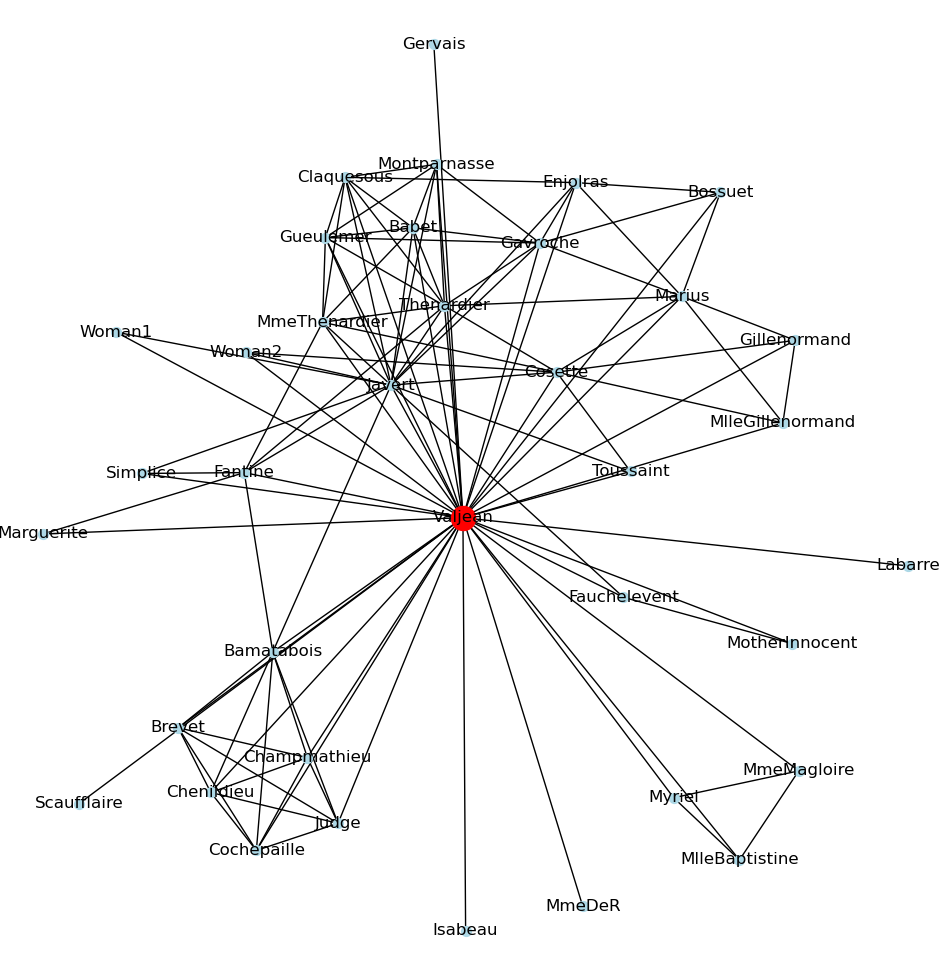
\includegraphics[width=\linewidth]{./LesMis_ego_vis.png}
            \caption{lesmis ego graph}
            \label{fig:lesmis_gr}
        \end{figure}
        
        \begin{figure}
            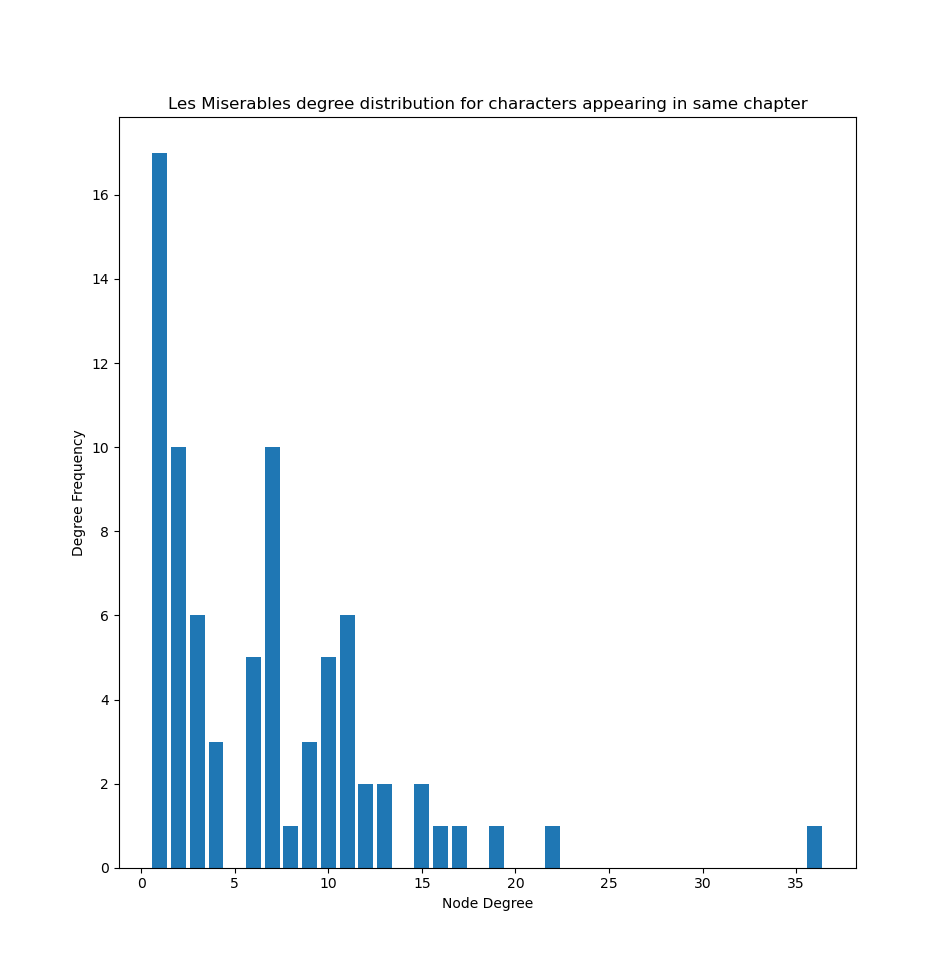
\includegraphics[width=\linewidth]{./LesMis_degree_dist.png}
            \caption{lesmis degree distribution}
            \label{fig:lesmis_deg}
        \end{figure}

        For the power dataset, I firstly used python and networkx to generate a csv file with the degree distribution, then plotted it using R with ggplot2. I also used R to analyze the data. Firstly, I plotted the log-log graphs as shown in Fig. \ref{fig:power_loglog}. This fit wasn't linear enough to deem correct, and so I moved on to a log- plot as in Fig. \ref{fig:power_log}, which clearly showed a linear behaviour in the subset of degrees [2, 14]. From this, I extracted the exponential behaviour as $\exp(8.25-0.528* degree) $. Fig. \ref{fig:power_vis} shows that there are a large number of "leaf" nodes, namely, nodes which only connect to one other node.  

        \begin{figure}
            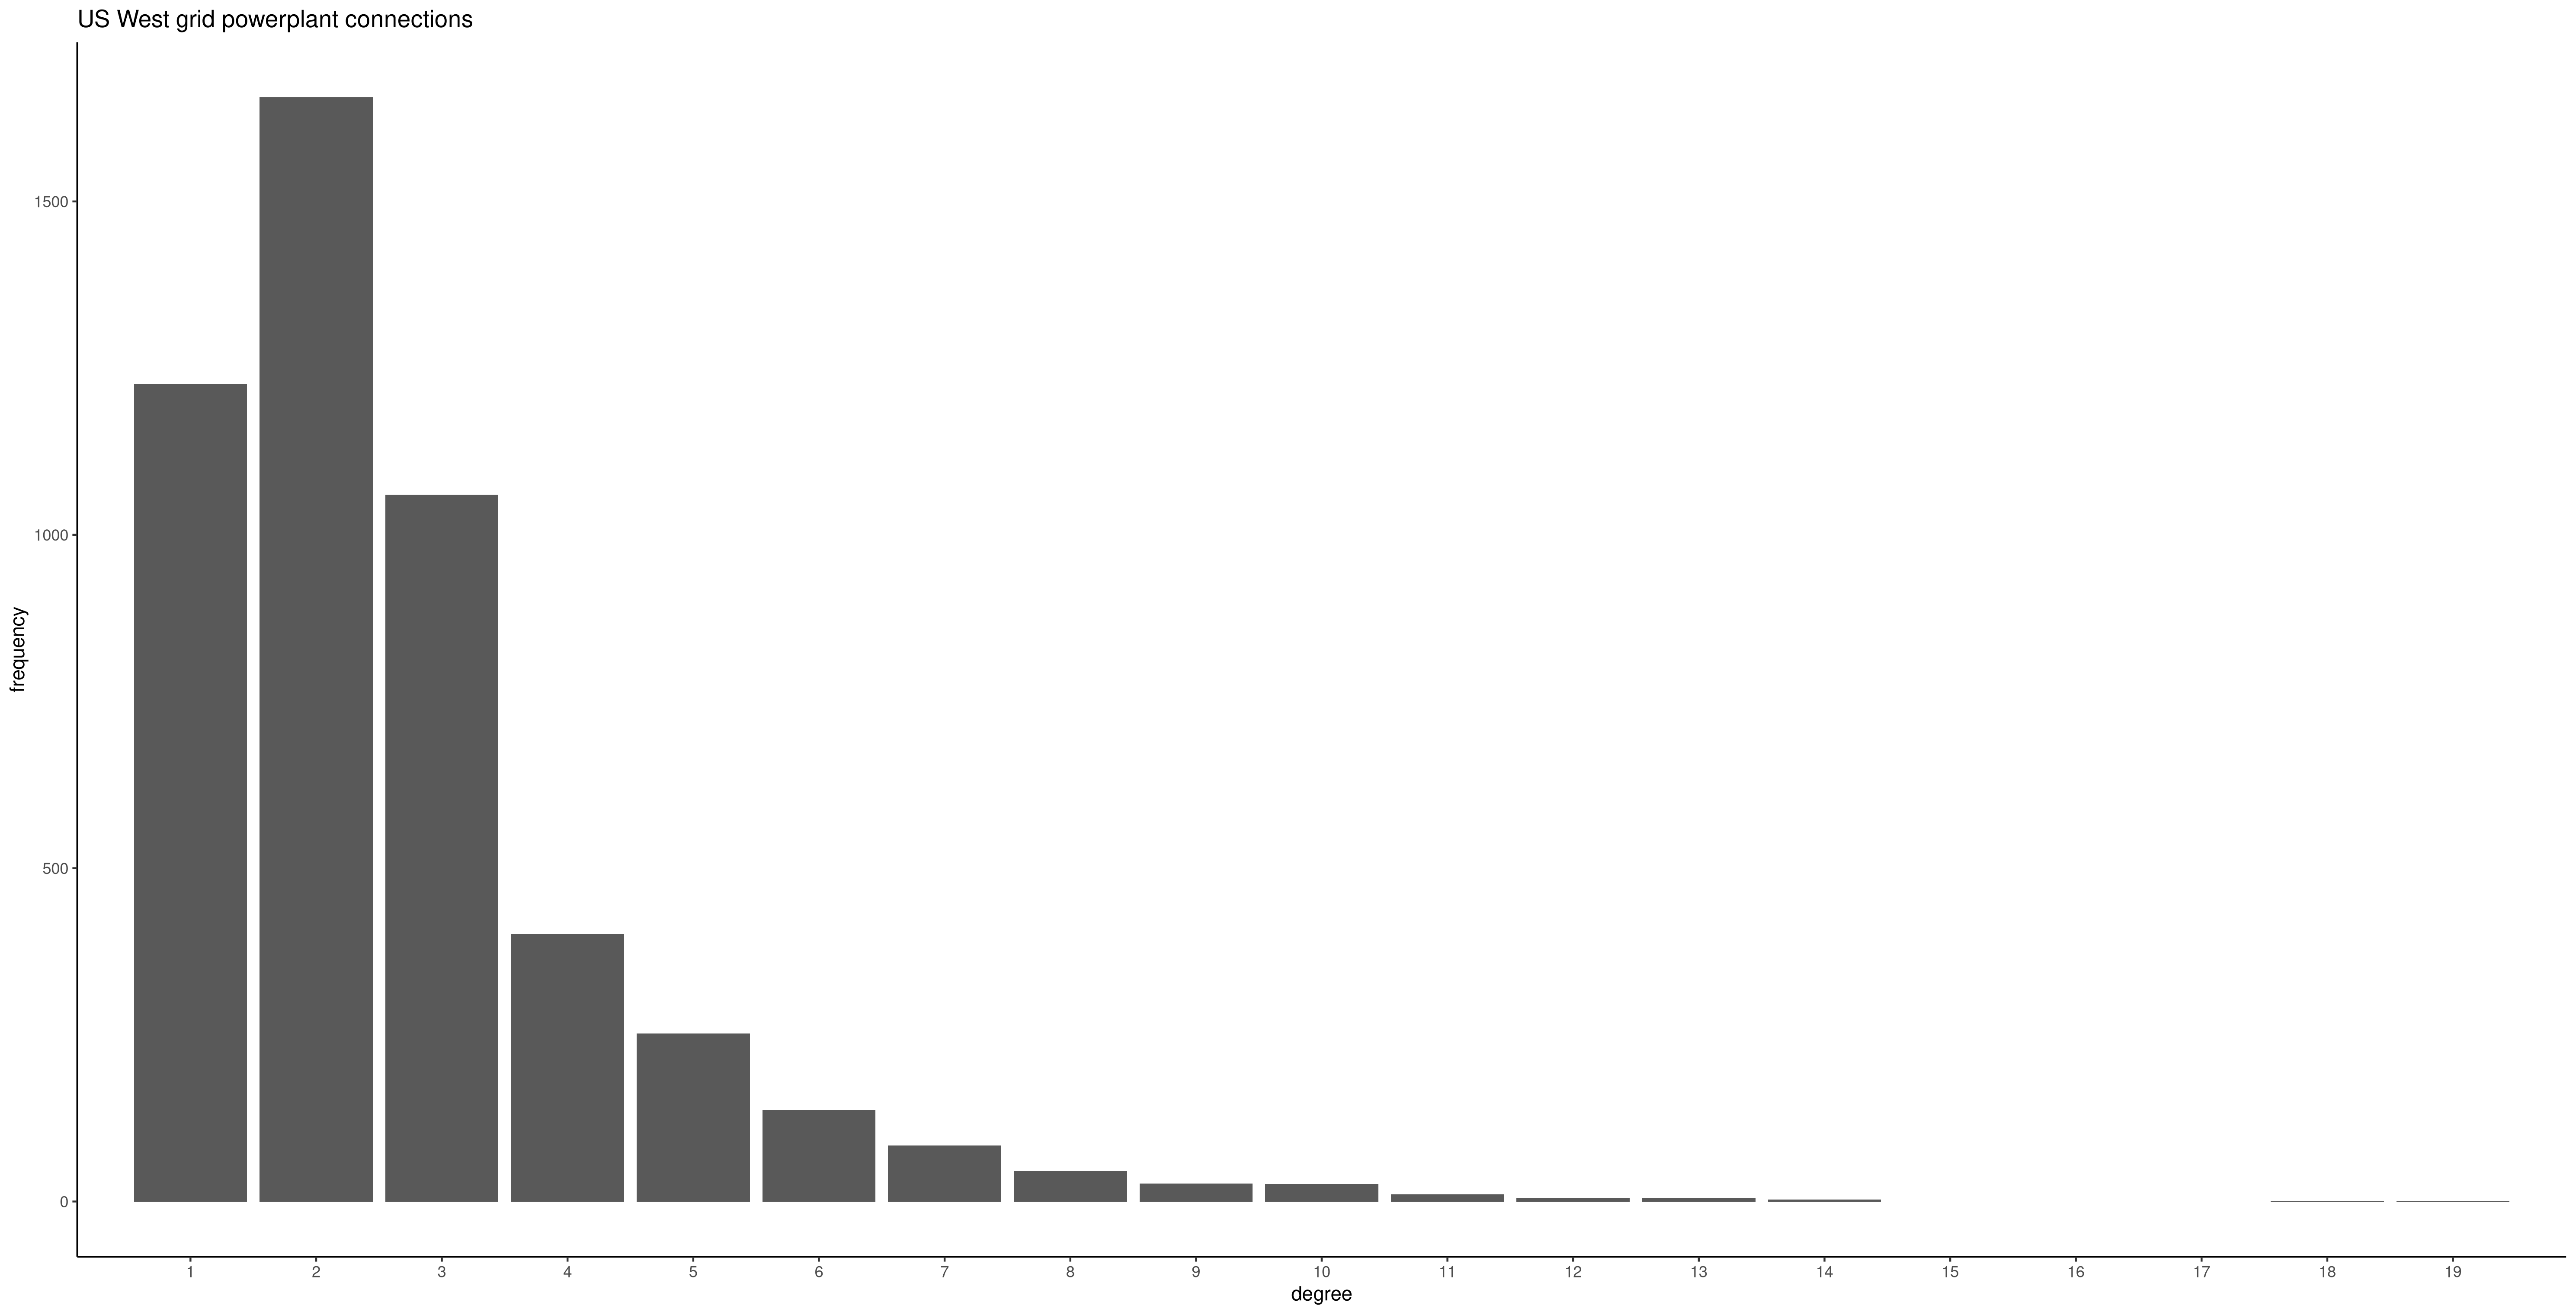
\includegraphics[width=\linewidth]{./power_degree_dist.png}
            \caption{power degree distribution}
            \label{fig:power_deg}
        \end{figure}

        \begin{figure}
            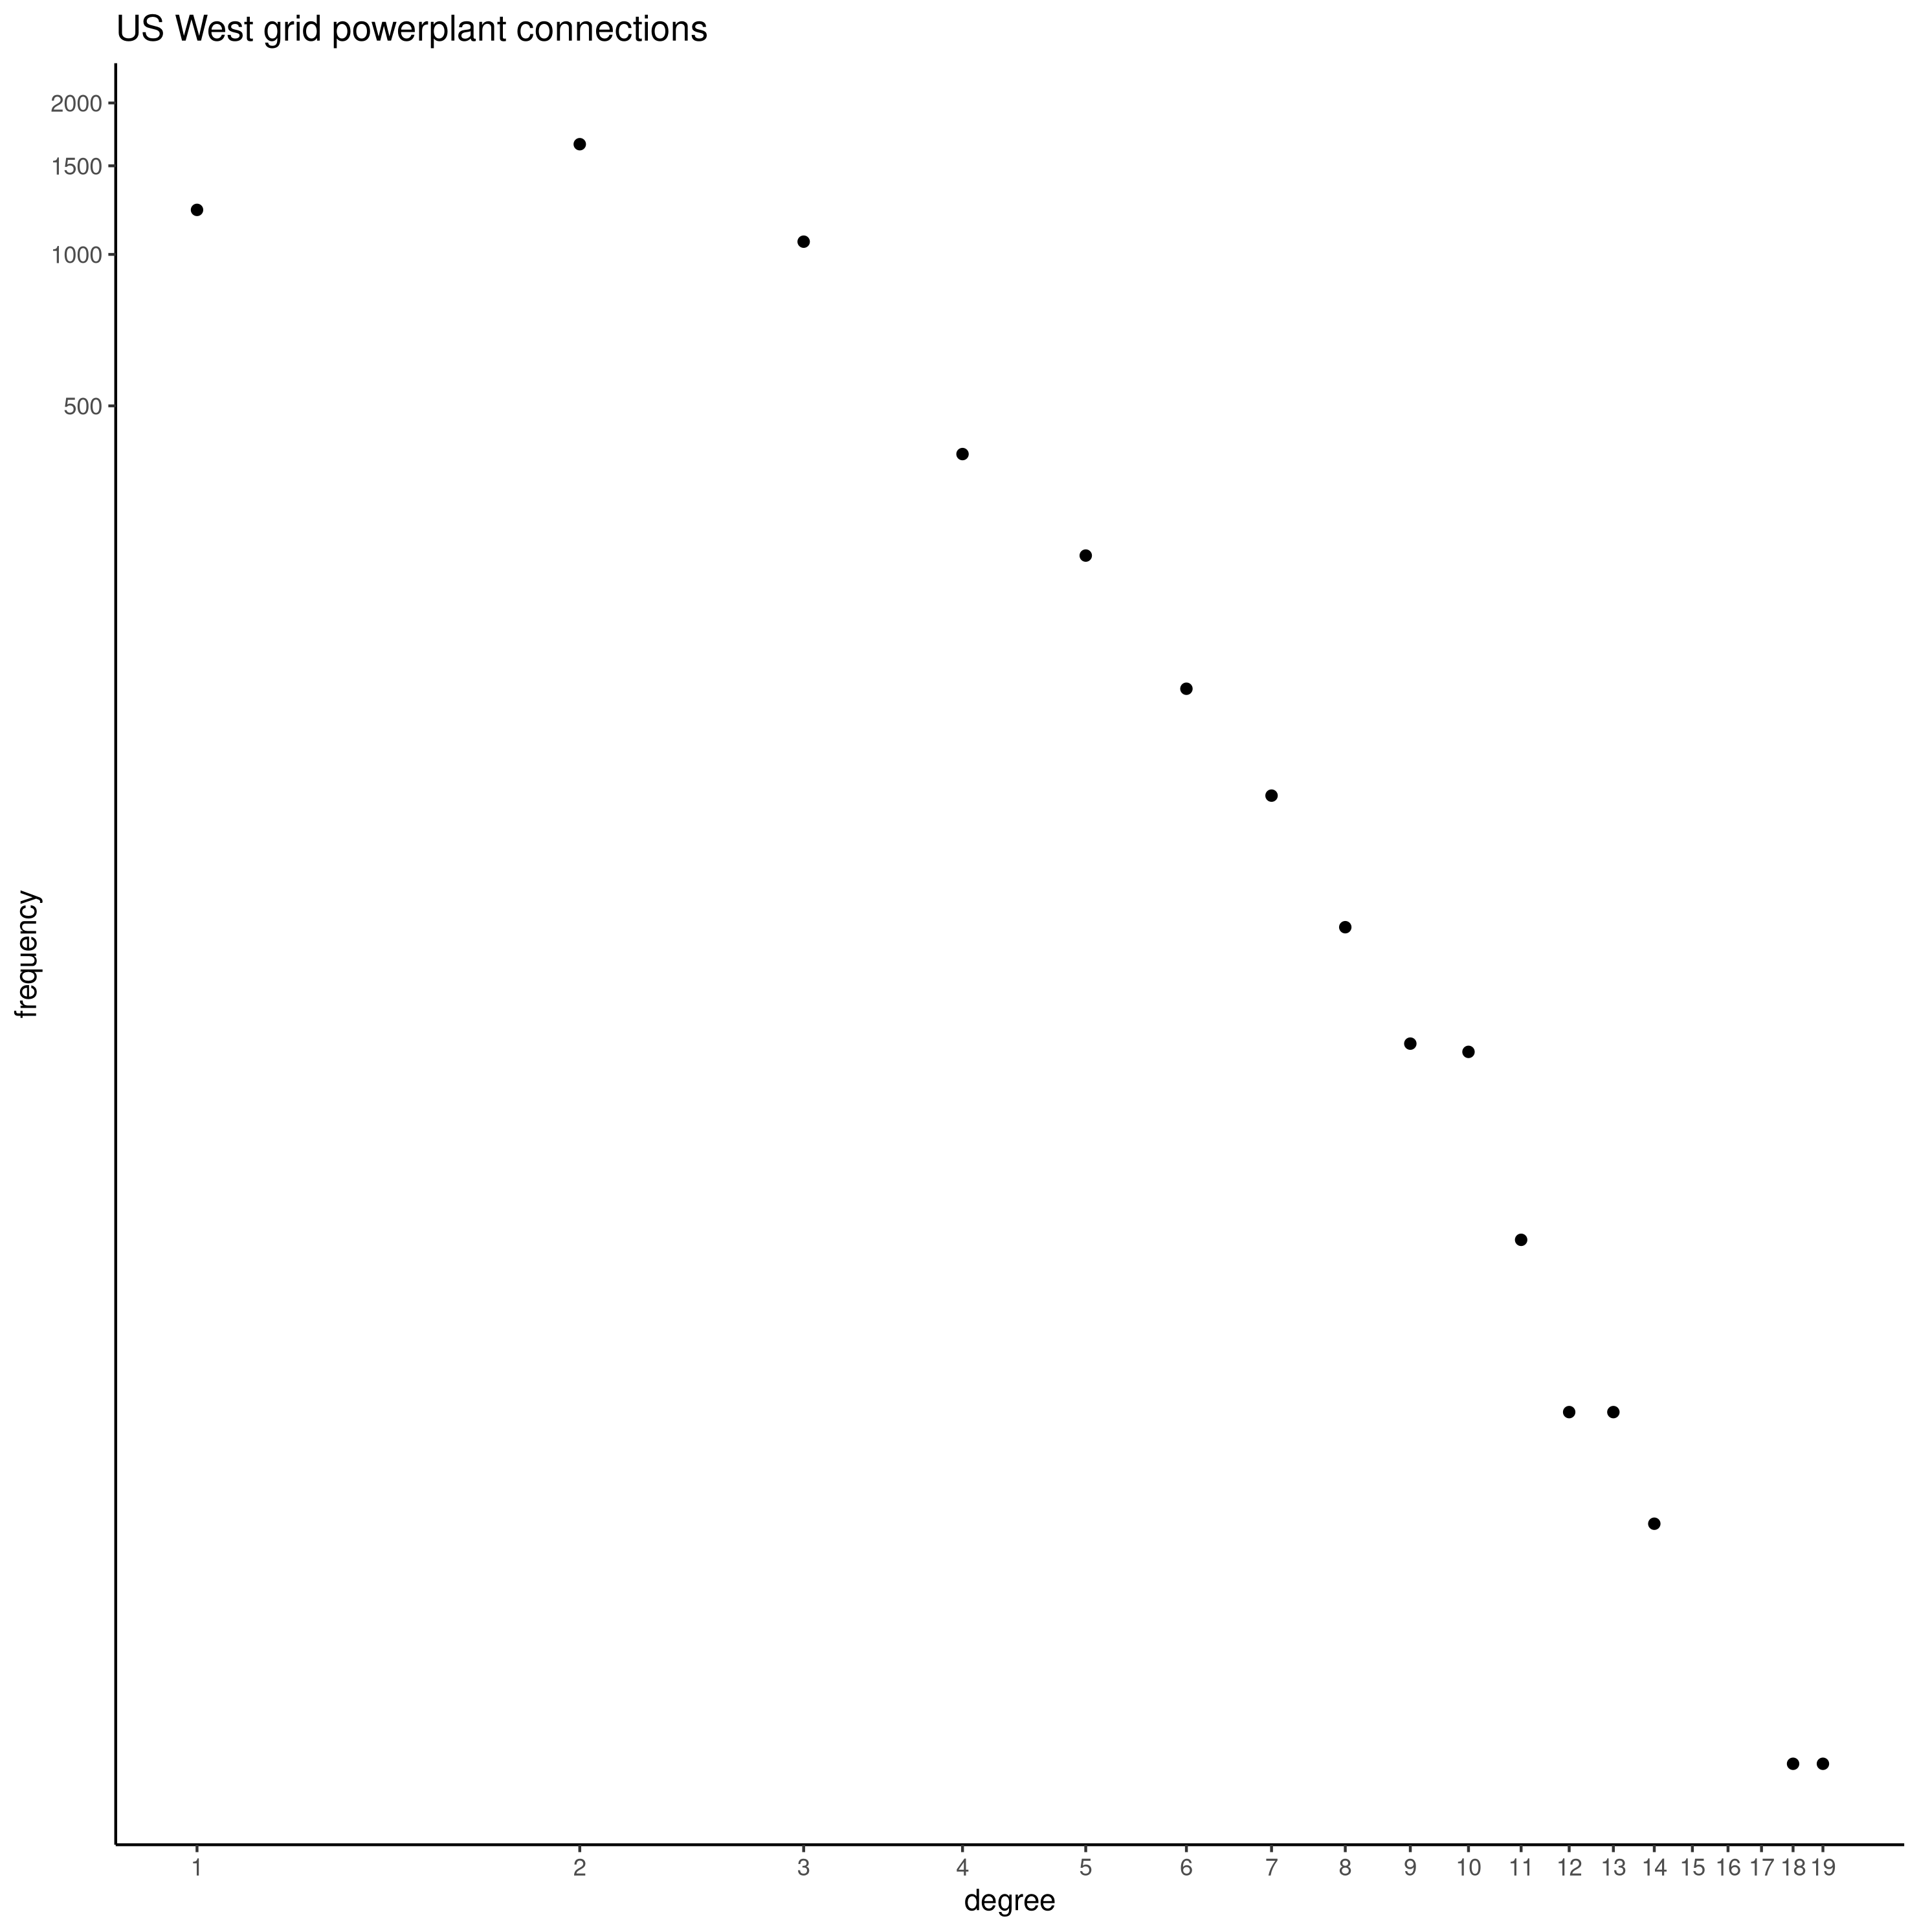
\includegraphics[width=\linewidth]{./power_deg_dist_loglog.png}
            \caption{power degree distribution}
            \label{fig:power_loglog}
        \end{figure}

        \begin{figure}
            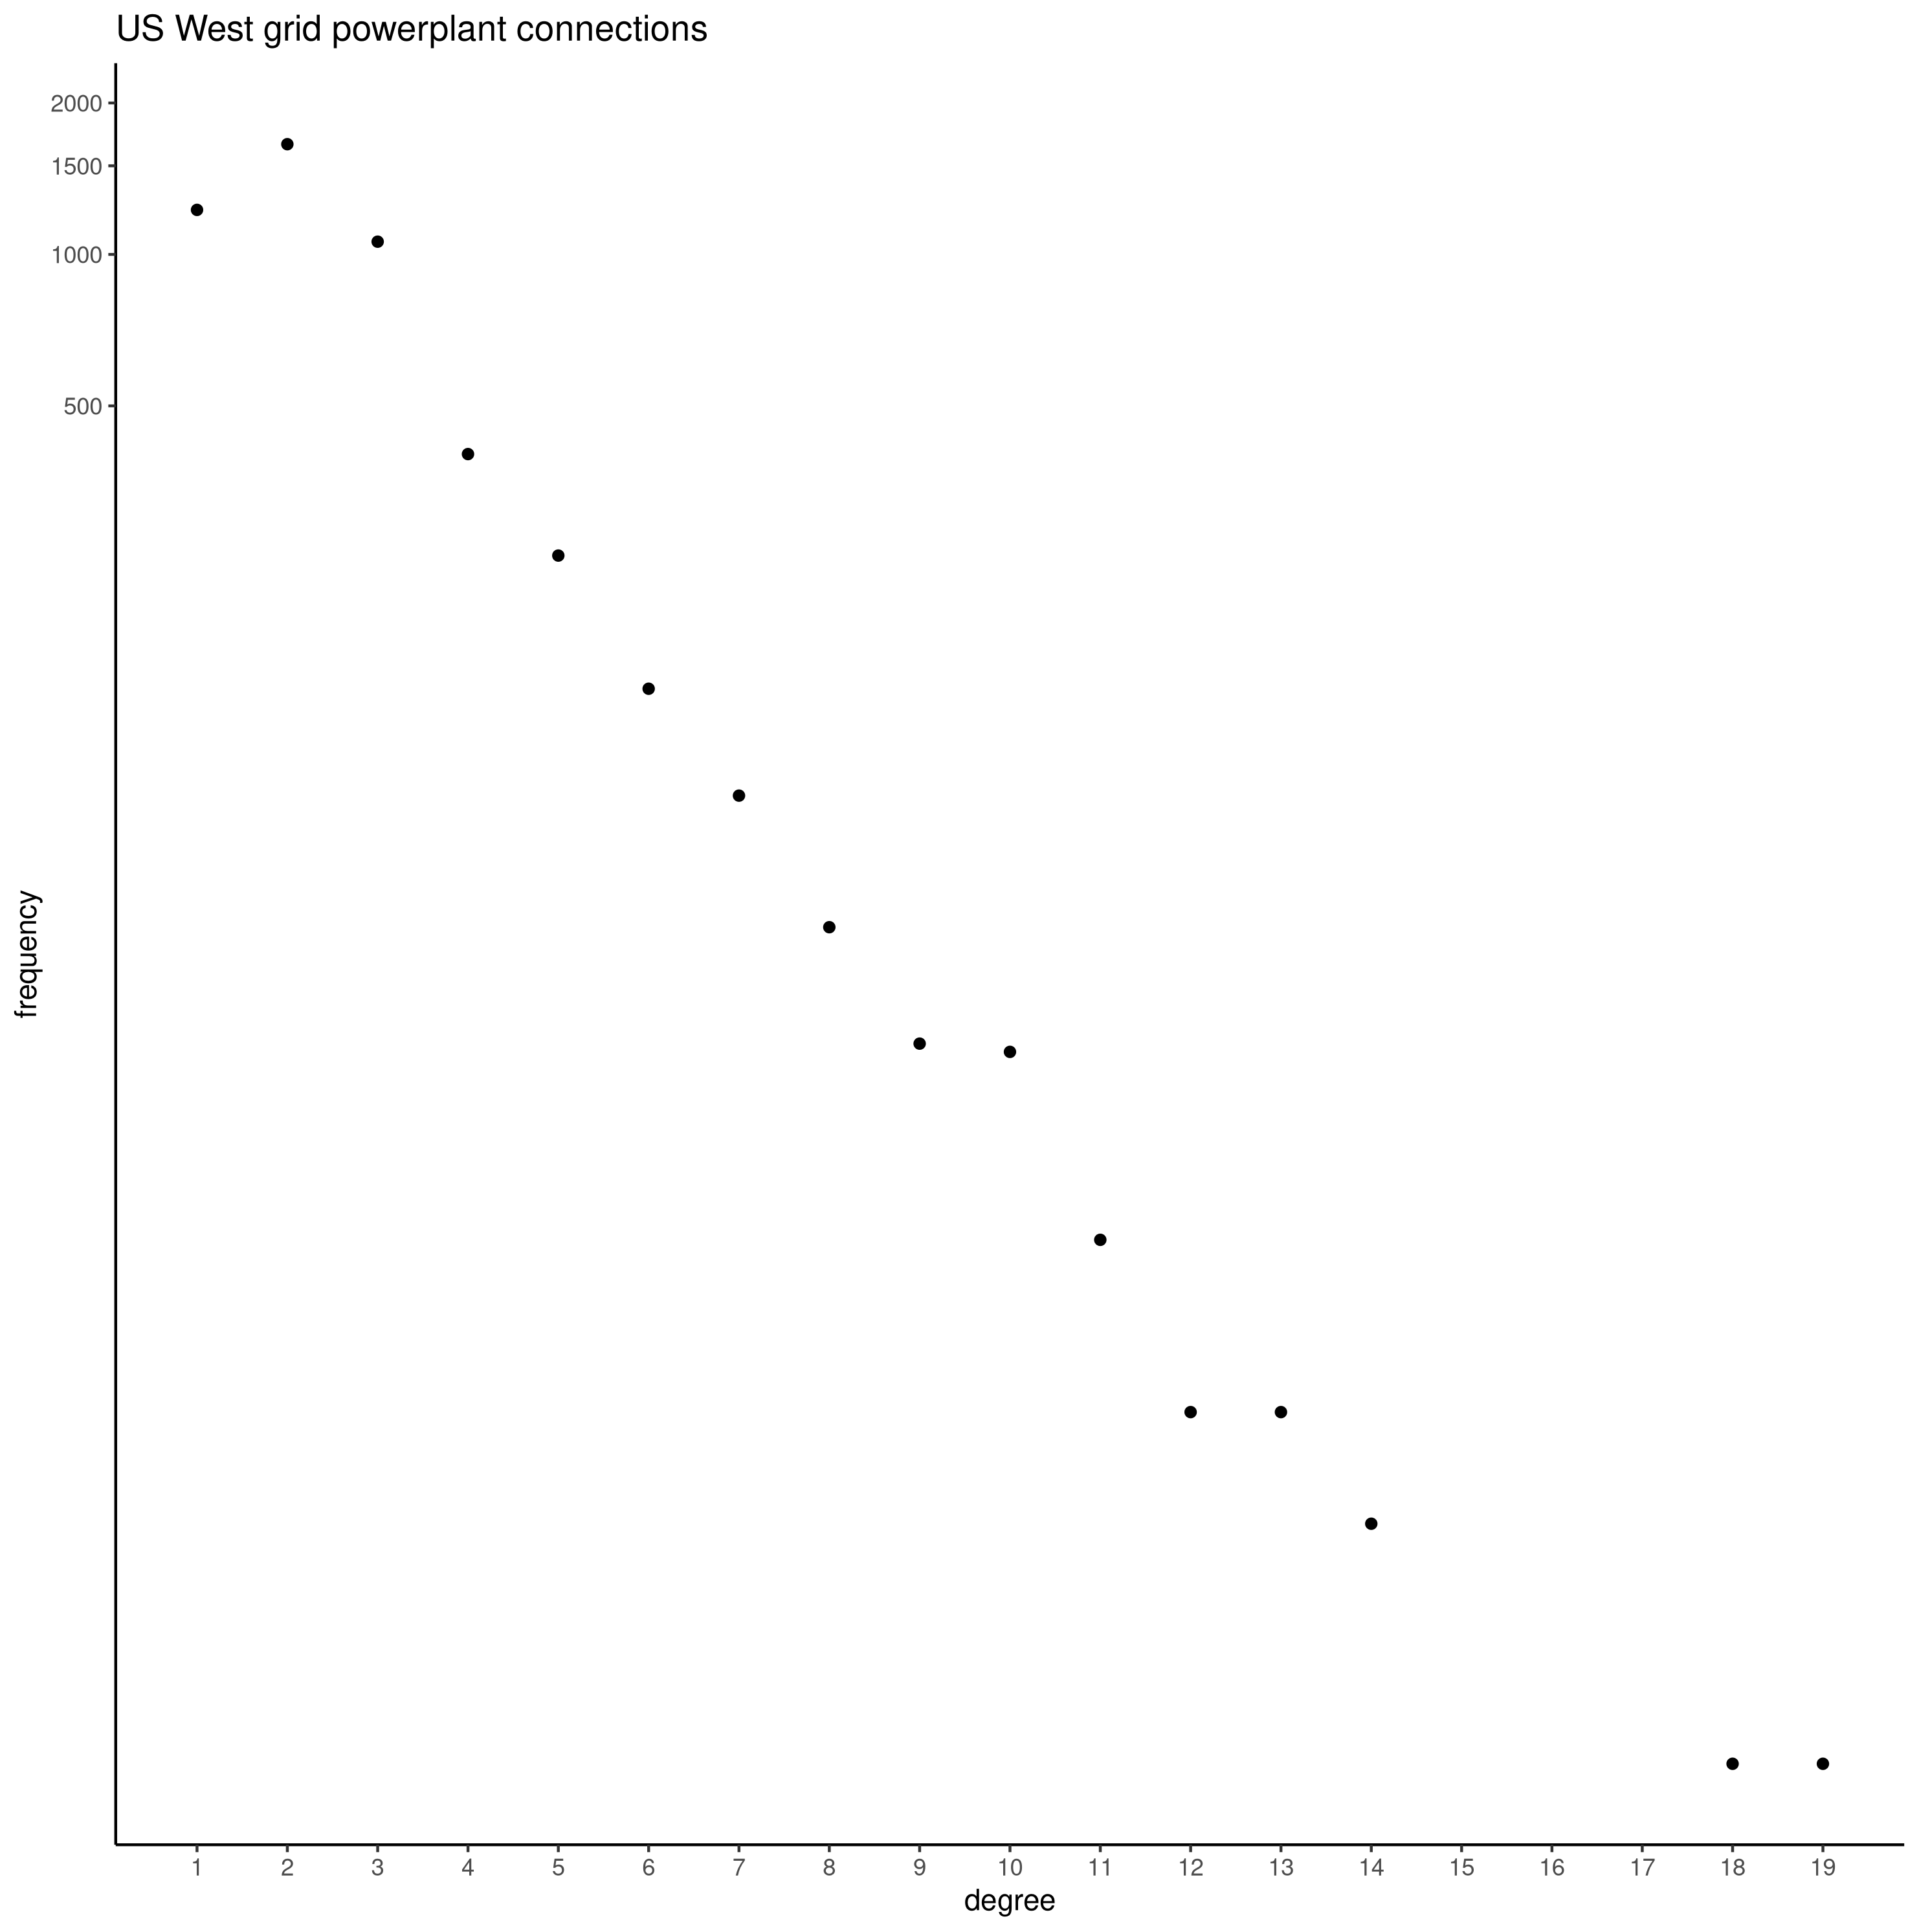
\includegraphics[width=\linewidth]{./power_deg_dist_log.png}
            \caption{power degree distribution}
            \label{fig:power_log}
        \end{figure}

        \begin{figure}
            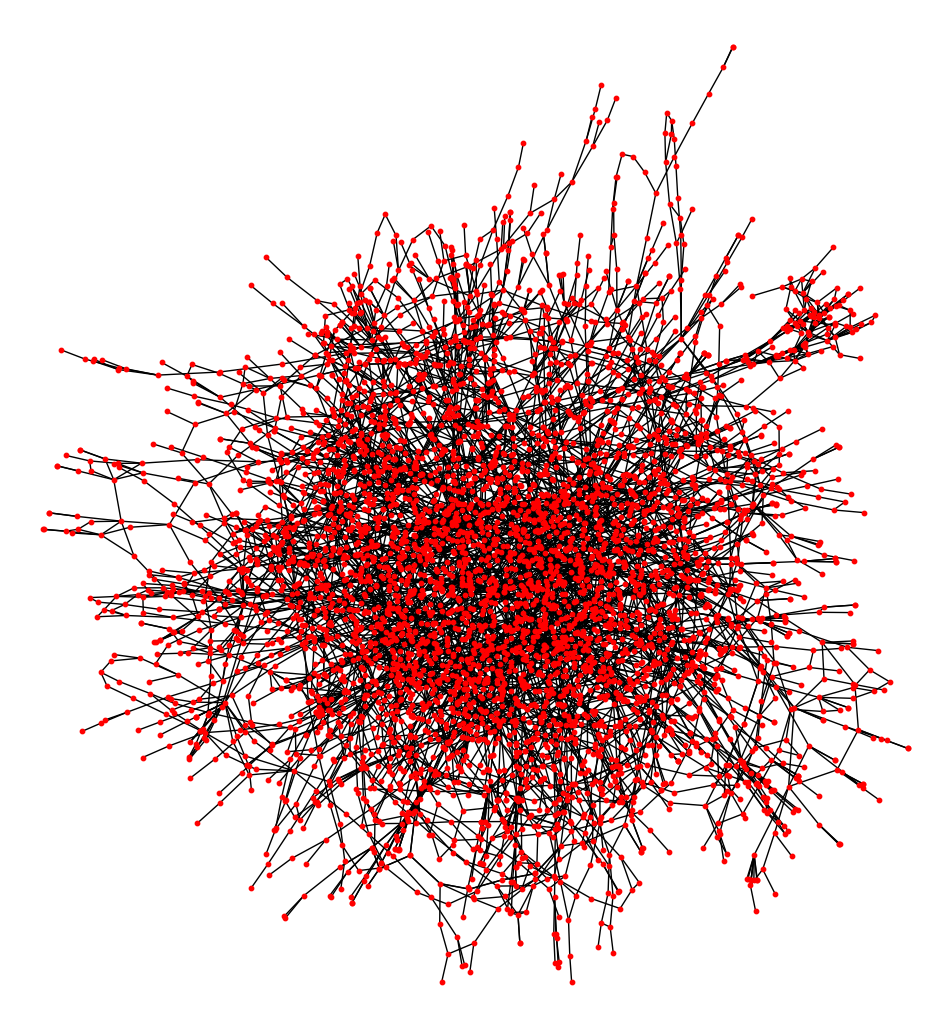
\includegraphics[width=\linewidth]{./power_vis.png}
            \caption{power network visualization}
            \label{fig:power_vis}
        \end{figure}

\end{enumerate}

\section{Mathematical Toolbox}

\begin{enumerate}[label={(2. \alph*)}]
    \item
        Fig. \ref{fig:bern} shows that the computed variance matches the mathematics. The mean was computed to be $p$. 
        \begin{figure}
            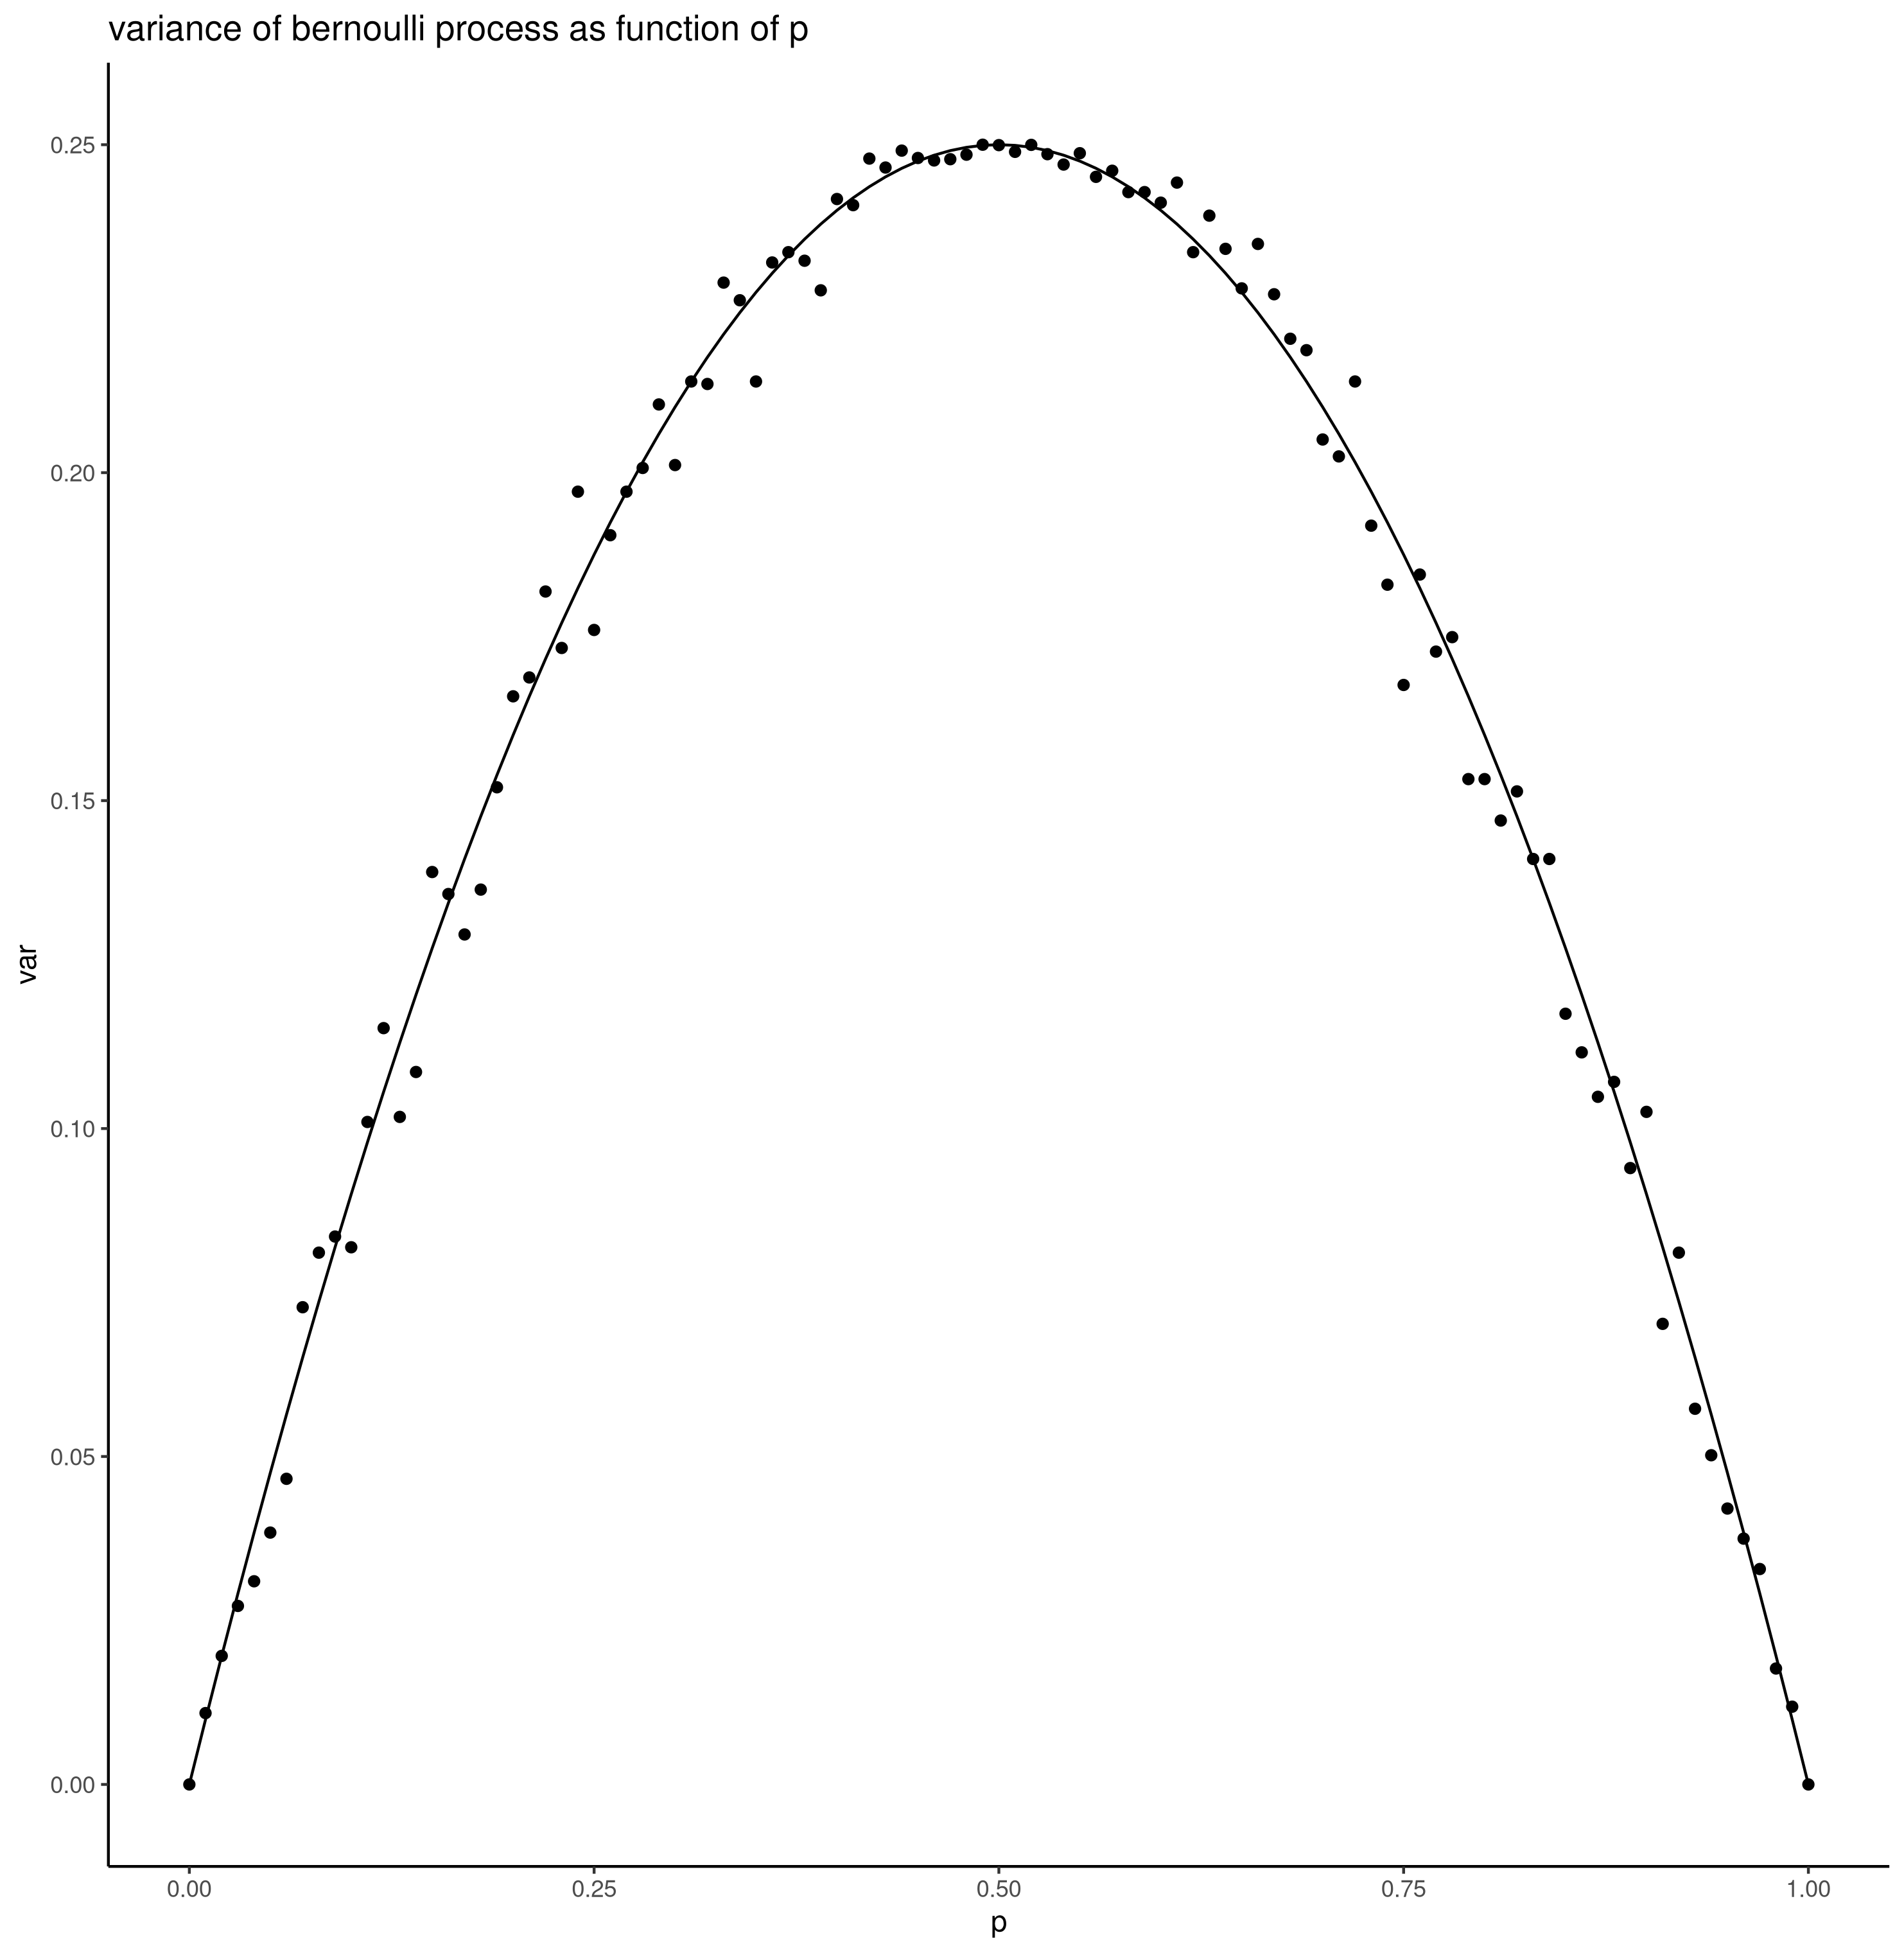
\includegraphics[width=\linewidth]{./bernoulli_var.png}
            \caption{bernoulli process variance, with overlayed $p(1-p)$:}
            \label{fig:bern}
        \end{figure}
    \item
        I simulated 10000 random walkers and plotted the resulting position distribution for 5000, 10000 and 15000 samples. From theory (the notes), we know the data should follow the gaussian profile \[
            p(x;t) = \frac{1}{\sqrt{2 \pi D t}} \exp{\frac{-x^2}{4 D t} 
        .\] With D given by,
        \[
            D = \frac{\langle x^2 \rangle}{2} = \frac{1}{2}
        .\] With this, the data didn't fit, as the gaussian is not normalized properly. The correct normalisation should be, for continuous data $\frac{1}{\sqrt{4\pi D t}}$. (Is this a problem with the notes?) With this normalisation, our gaussian is at half of the amplitude of the data, and that's because at any given iteration, we can only access either the even-, or odd-numbered positions. Thus, we are overcompensating and need to multiply by two. Thus, for our data, the correct normalisation is 
        \[
            p(x;t) = \frac{1}{\sqrt{\pi D t}} \exp{\frac{-x^2}{4 D t}} 
        .\]   
        Figs. \ref{fig:rw5000}, \ref{fig:rw10000}, \ref{fig:rw15000} show the data fitting to the modified gaussian correcly. 

        \begin{figure}
            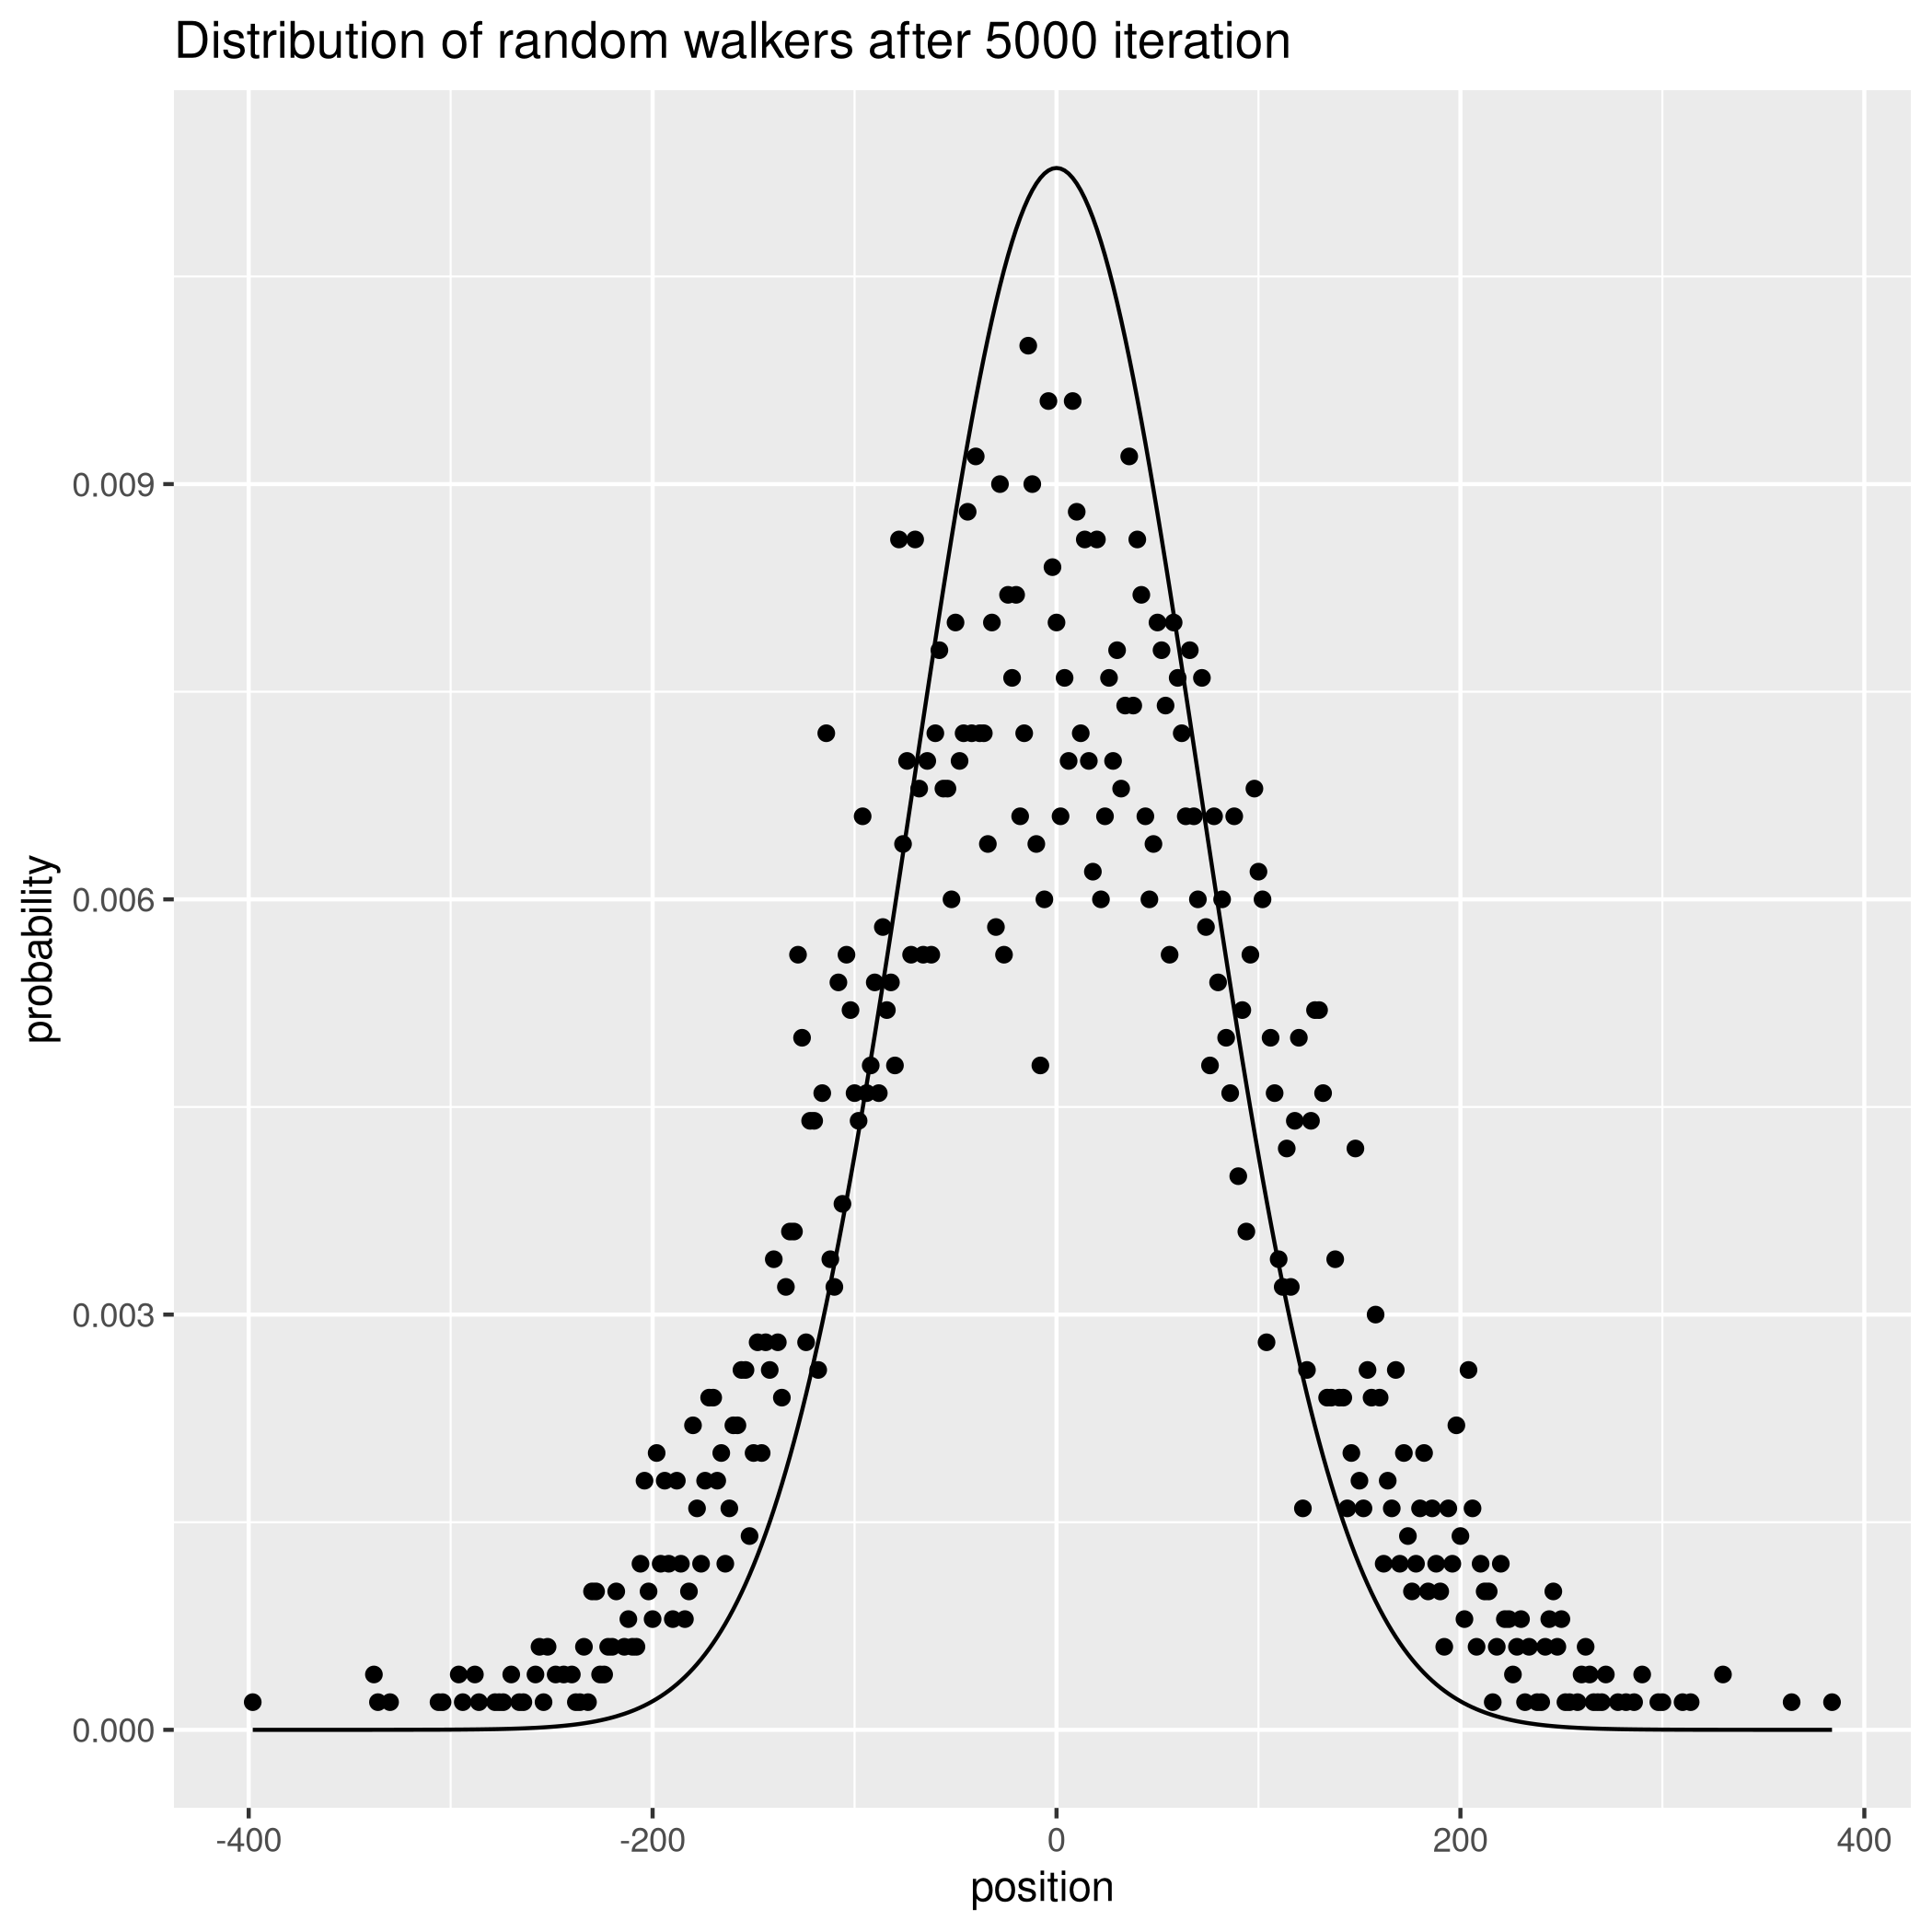
\includegraphics[width=\linewidth]{./random_walk5000.png}
            \caption{random walk after 5000 iterations}
            \label{fig:rw5000}
        \end{figure}
        \begin{figure}
            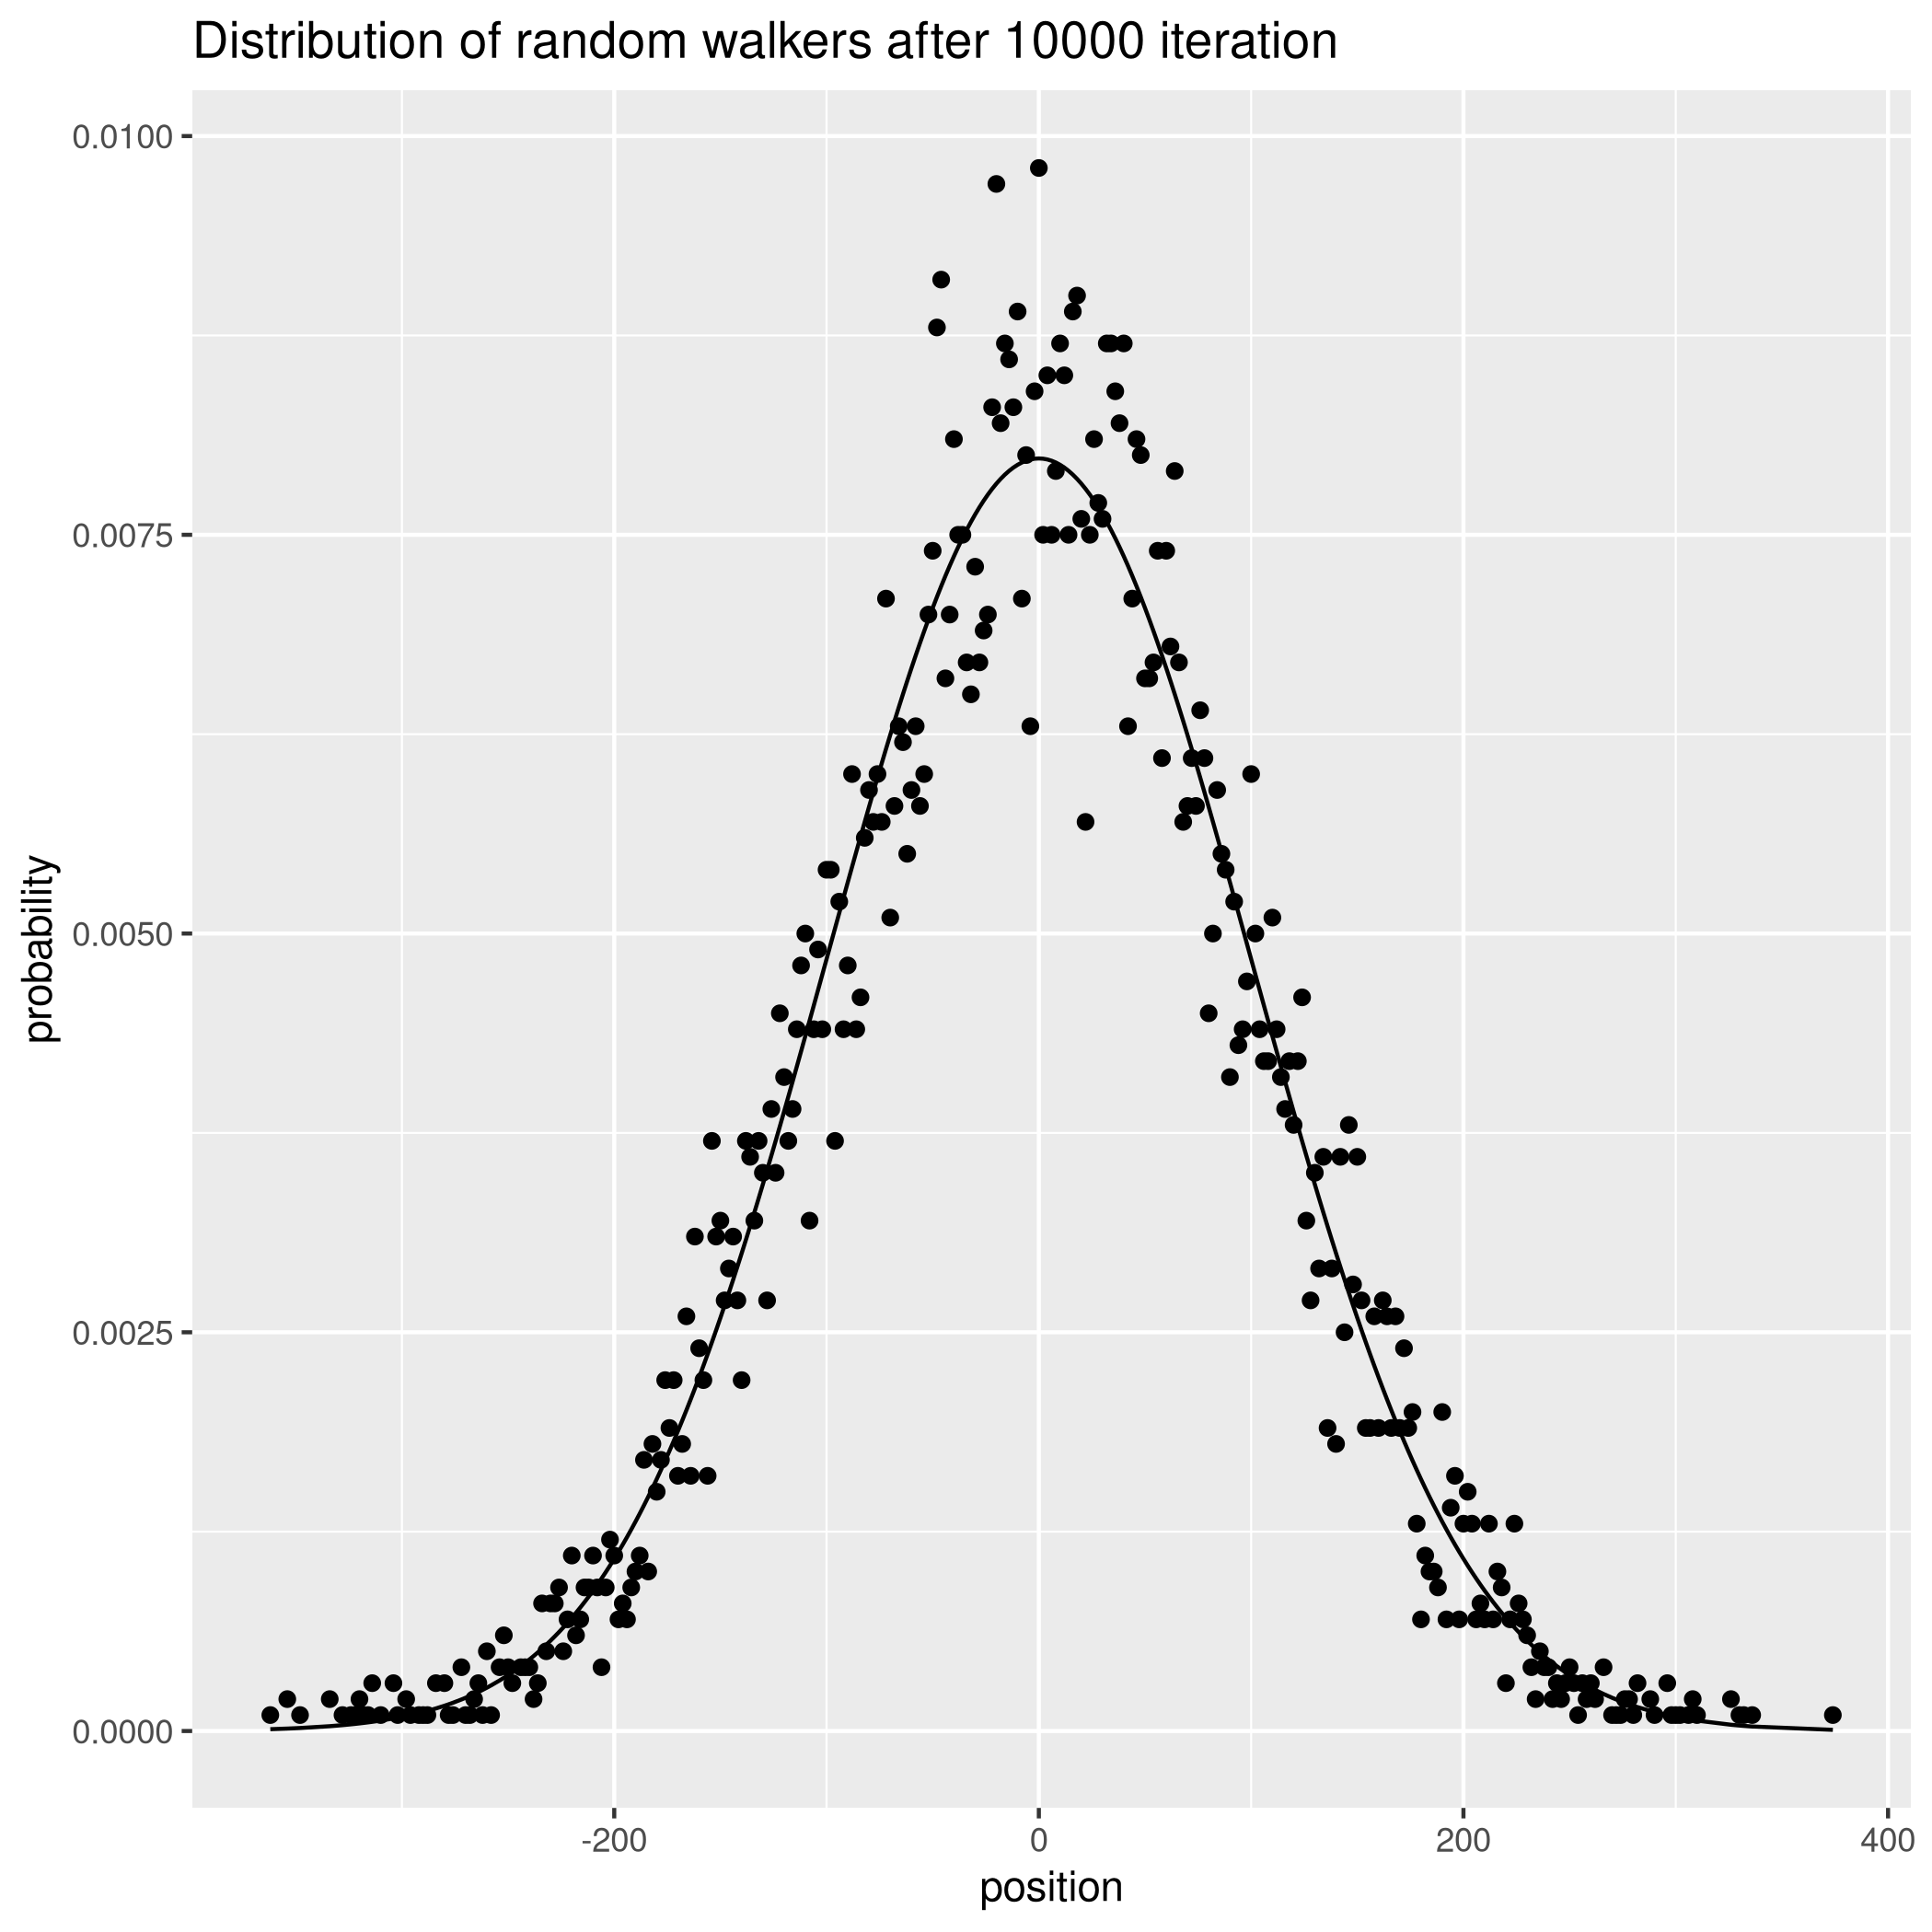
\includegraphics[width=\linewidth]{./random_walk10000.png}
            \caption{random walk after 10000 iterations}
            \label{fig:rw10000}
        \end{figure}
        \begin{figure}    
            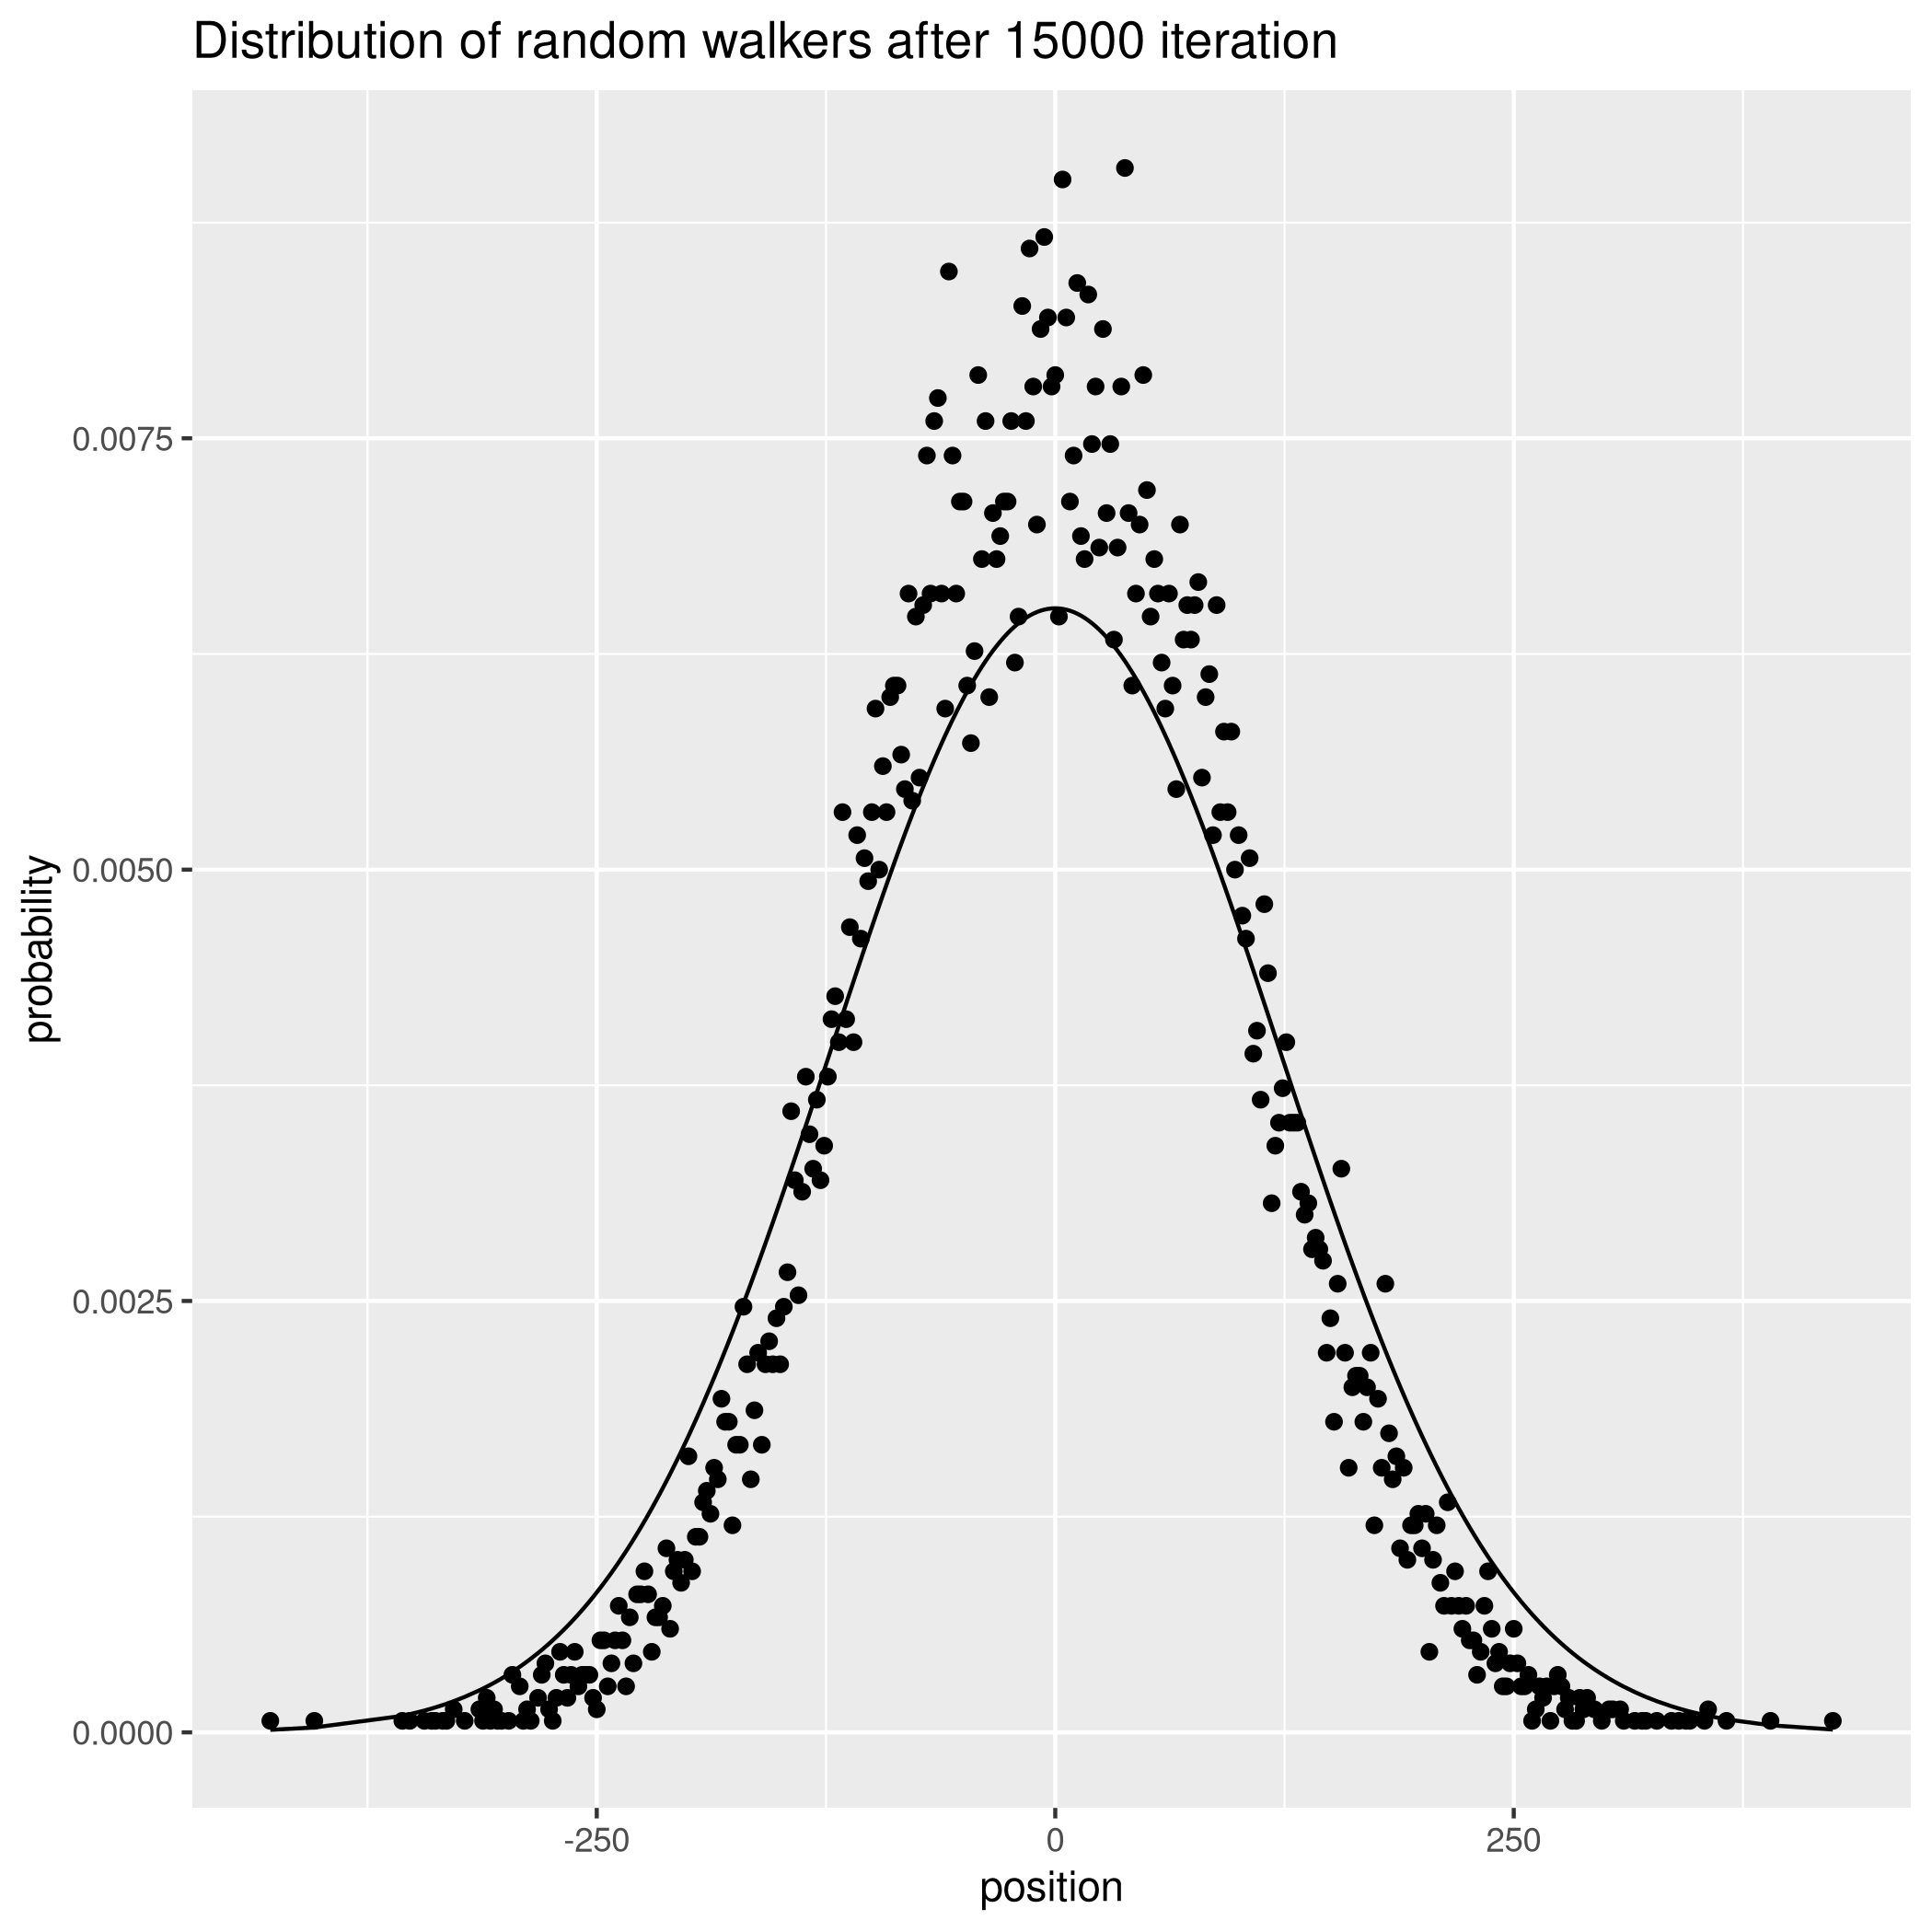
\includegraphics[width=\linewidth]{./random_walk15000.png}
            \caption{random walk after 15000 iterations}
            \label{fig:rw15000}
        \end{figure}
    \item
        Generating the matrices I found the distribution shown in Figs. \ref{fig:eig_dist_small}, \ref{fig:eig_dist_big}. The distribution looks like a semi-circle.
        \begin{figure}
            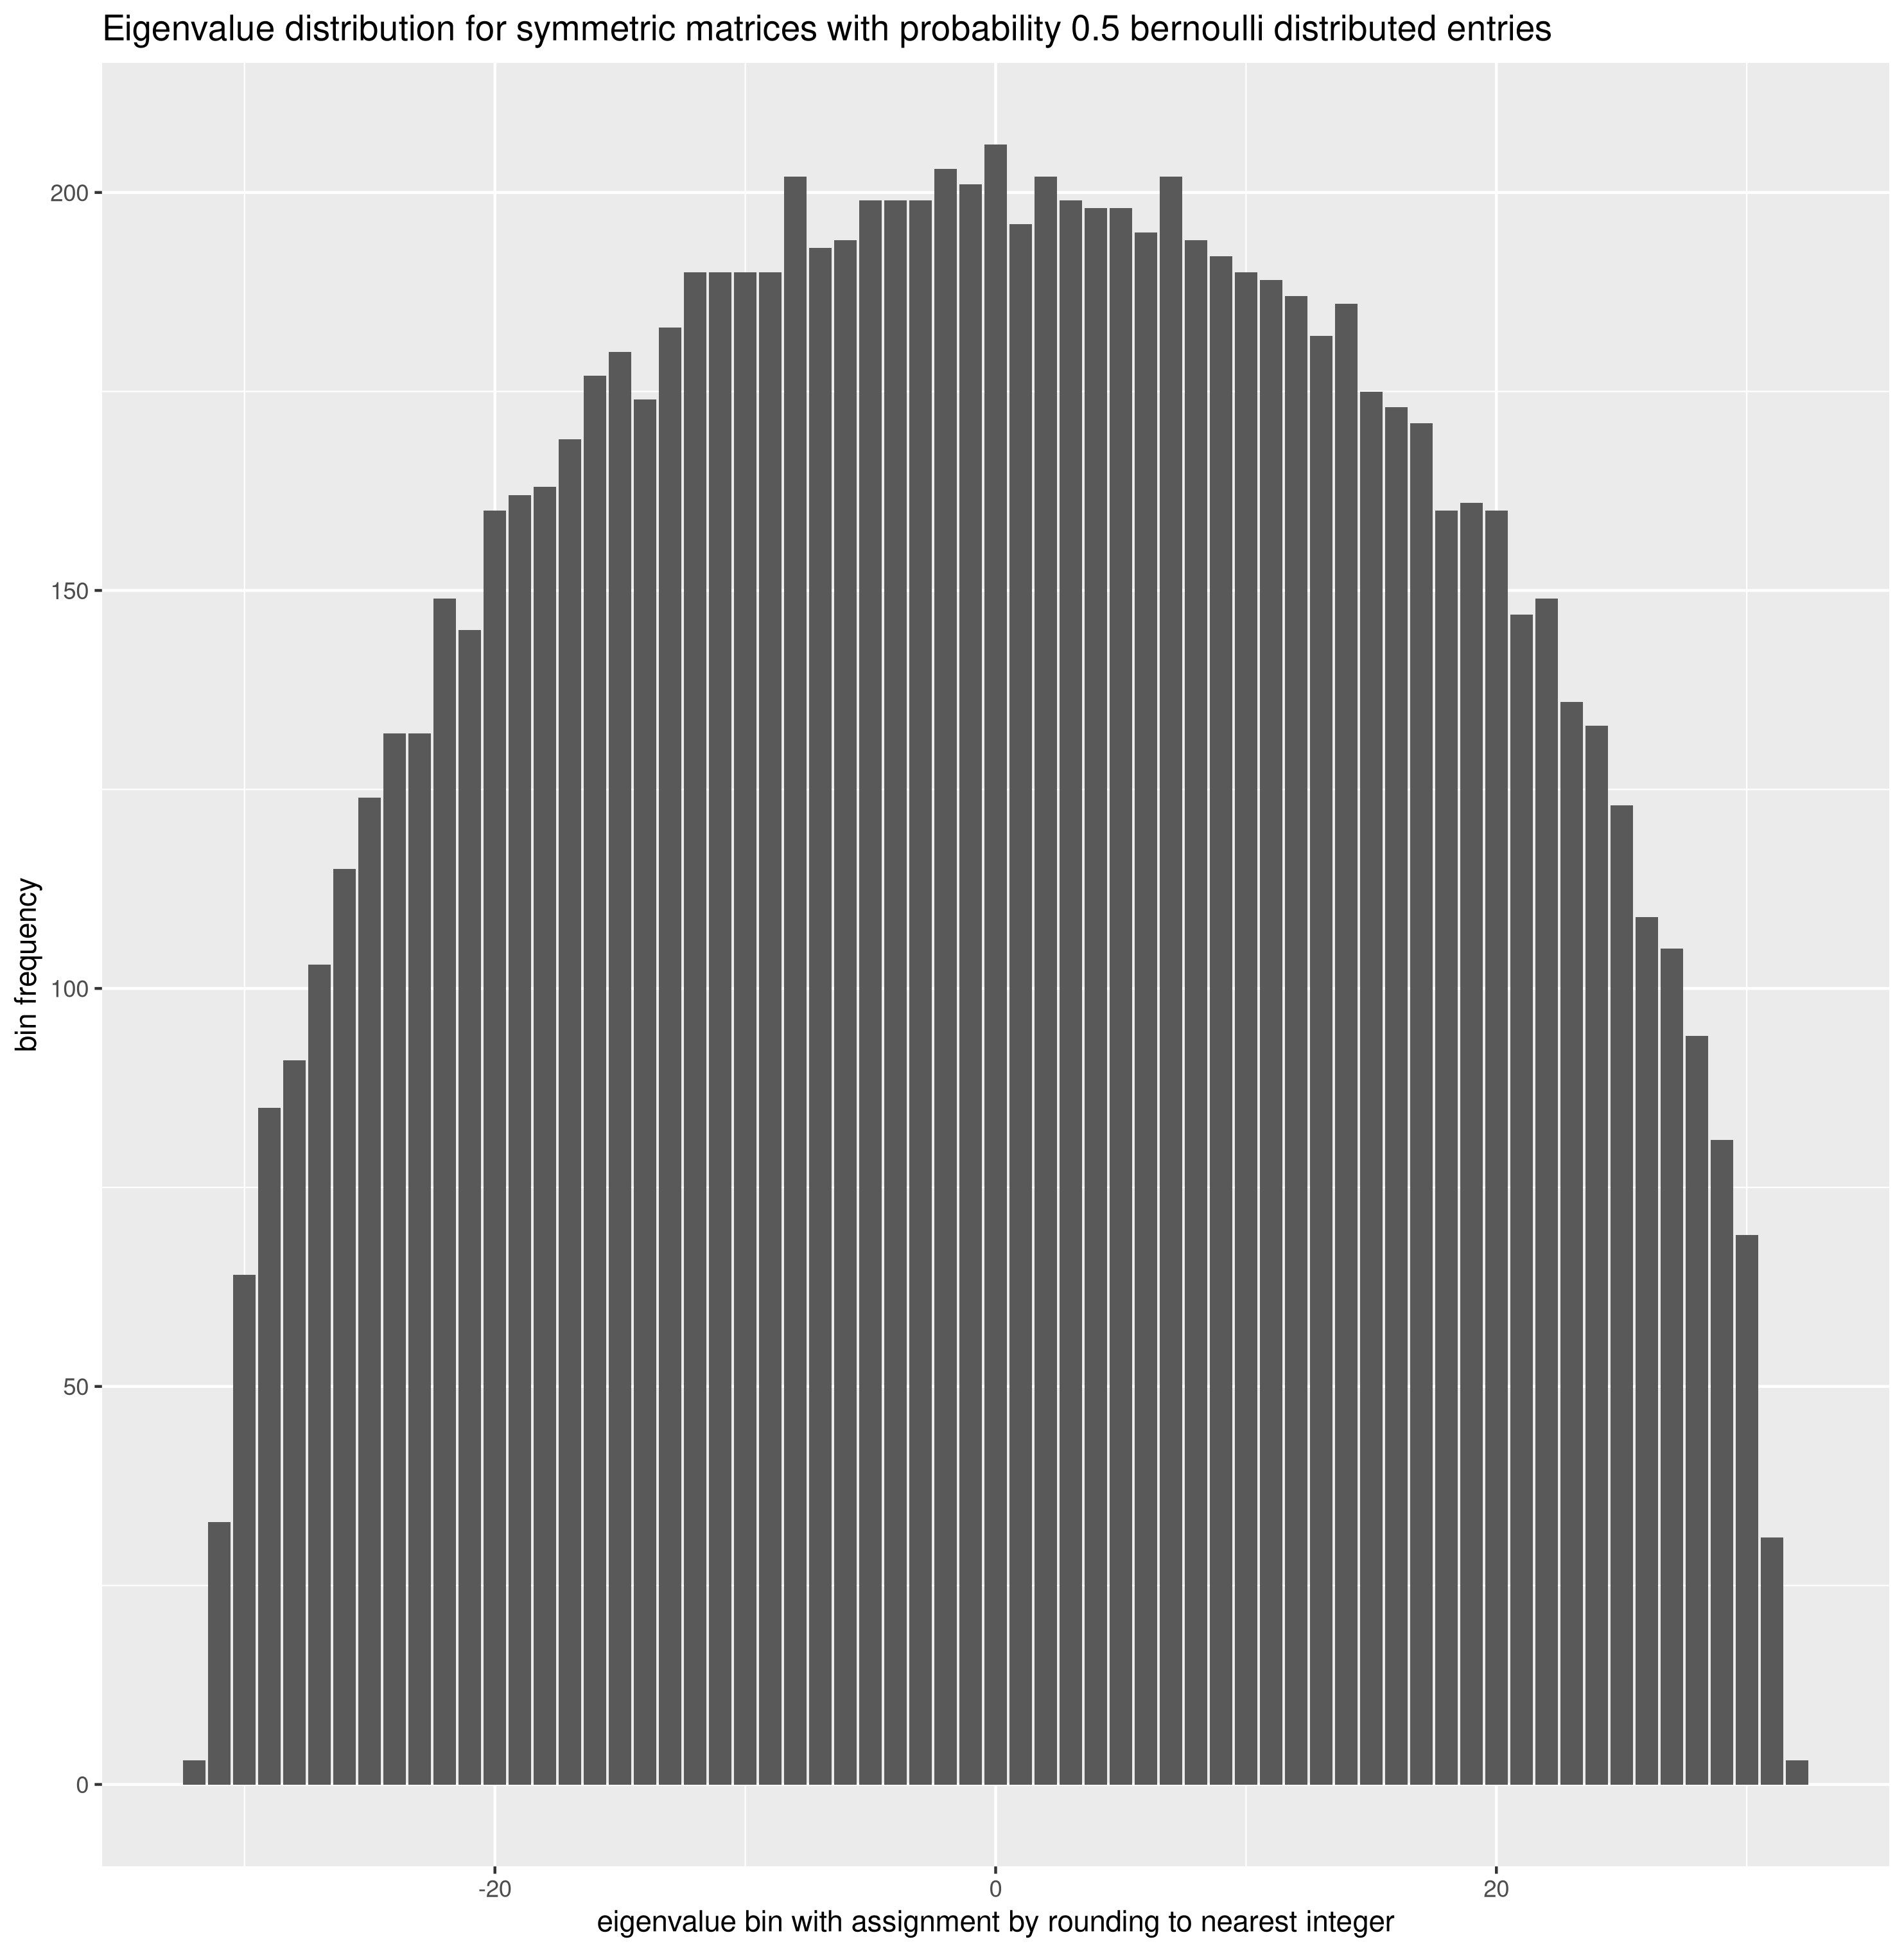
\includegraphics[width=\linewidth]{./eig_dist_small.png}
            \caption{Eigenvalue distribution for bin < 100}
            \label{fig:eig_dist_small}
        \end{figure}
        \begin{figure}
            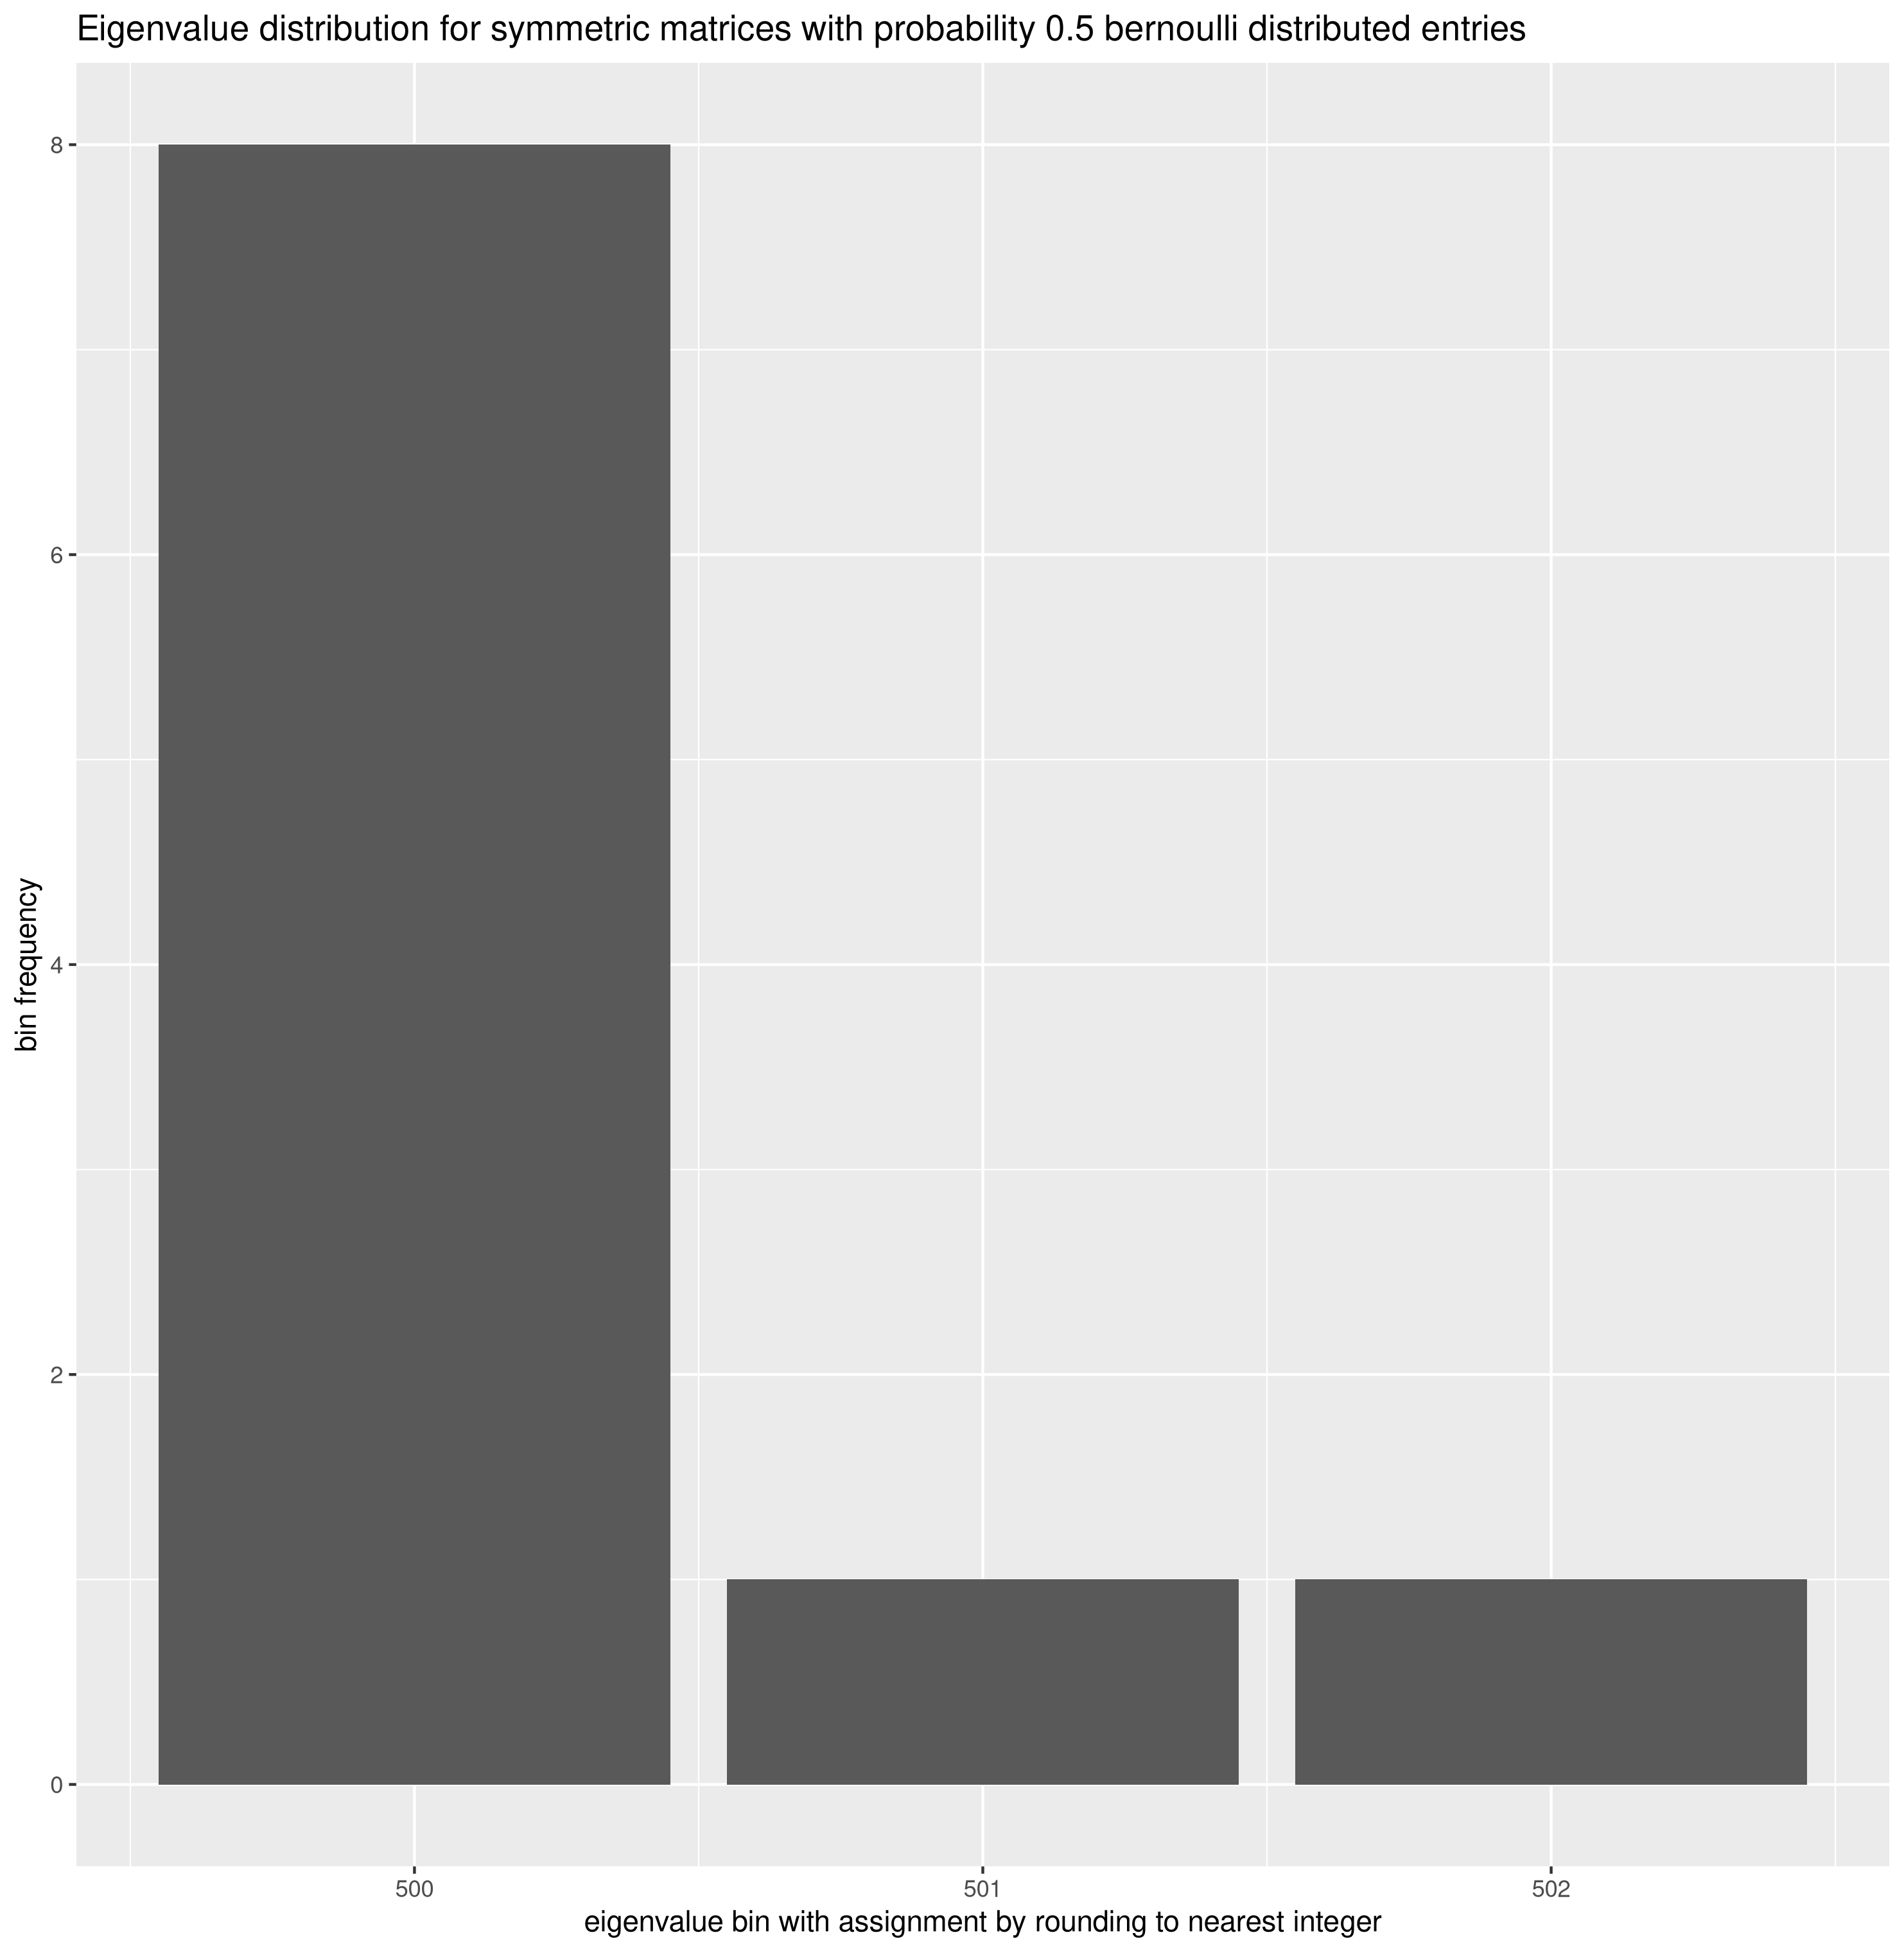
\includegraphics[width=\linewidth]{./eig_dist_big.png}
            \caption{Eigenvalue distribution for bin > 100}
            \label{fig:eig_dist_big}
        \end{figure}

\end{enumerate}

\section{Connectedness}

\bibliography{citations}

\end{document}
